%\documentclass[a4paper,12pt,twoside]{book}
\documentclass[12pt,times]{report}
\usepackage{mathptmx}%This package supersedes times and mathptm
\usepackage[a4paper,right=2.54cm,left=2.54cm,top=2.54cm,bottom=2.54cm]{geometry}

%%%%paquete para usar citas de diferentes formatos
%%%%%%%%%%%%%%%%%%%%%%%%%%%%%%%%%
%%add al indice
%\usepackage[nottoc,numbib]{tocbibind}
%\usepackage[authoryear,round]{natbib}
\usepackage[utf8]{inputenc}
\usepackage{csquotes}
\usepackage[spanish]{babel}
\usepackage[style=apa ,
%hyperref=auto,
%citestyle=authoryear,
natbib=true,
backend=biber]{biblatex}
\addbibresource{biblio/references.bib}
%\usepackage{biblatex}
%paquete para hiperlinks entre citas e imagenes
%%%%%%%%%%%%%%%%%%%%%%%%%%%%%%%%%
\usepackage[colorlinks=true,
citecolor=blue,
urlcolor=cyan,
bookmarks=true,
linkcolor=blue,
pdftitle={Tesis-nombre-alumno},
pdfauthor={autor nombres}]{hyperref}

\usepackage{amssymb}
\usepackage{graphicx} % for improved inclusion of graphics
%\usepackage{wrapfig} % to include figure with text wrapping around it
\usepackage[margin=10pt,font=small,labelfont=bf]{caption} % for improved layout of figure captions with extra margin, smaller font than text
\usepackage{eucal}
\usepackage[usenames, dvipsnames]{color}
\usepackage[perpage]{footmisc}
%\usepackage[round, sort]{natbib}
\usepackage{ifthen}
\usepackage{multicol} % for pages with multiple text columns, e.g. References
\setlength{\columnsep}{20pt} % space between columns; default 10pt quite narrow
\usepackage[nottoc]{tocbibind} % correct page numbers for bib in TOC, nottoc suppresses an entry for TOC itself
\usepackage{appendix}

%%%----Modificar encabezado y pie de pagina
%%%%%%%%%%%%%%%%%%%%%%%%%%%%%%%%%%%%%%%%%%%%%%%%%%%%%%%%%%%%%%%%%%%%%
\usepackage{fancyhdr} % for better header layout
\newcommand{\changefont}{%
	\fontsize{9pt}{1.5pt}\selectfont
}
\pagestyle{fancy}
\fancyhf{} %% delete default configuration of page
%%\setlength\headheight{15pt}
%%\fancyhead[L]{\changefont Desarrollo de un sistema de detección haciendo uso de Deep Learning y visión por computadora para el Diagnóstico del Cáncer de Piel melanoma}
\fancyhead[R]{\changefont \leftmark}
%%\fancyfoot[L]{\leftmark}
\fancyfoot[R]{\thepage}

%%%%%%%%%%%%%%%%%%%%%%%%%%%%%5
%%%% Configuracion de los parrafos
%\usepackage{setspace}
%\onehalfspacing
%\linespread{1.25} 
\setlength{\parindent}{0.5in} %%sangria
\setlength{\parskip}{3mm}  %%espacio entre parrafos
\linespread{1.3} %This equals 1.5 linespacing in Word
%%%% nuevo parrafo
%%%%%%%%%%%%%%%%%%%%%%%%%%%%%5
%%%% Centrar valores de una tabla
\usepackage{array}
%%CENTRADO HORIZONTAL
\newcolumntype{P}[1]{>{\centering\arraybackslash}p{#1}}
%%CENTRADO VERTICAL
\newcolumntype{M}[1]{>{\centering\arraybackslash}m{#1}}

%%%%%%%%%%%%%%%%%%%%%%%%%%%%%5
%%%%Paquete para alinear texto
\usepackage{ragged2e}
\usepackage{multirow}
\usepackage{makecell}
\usepackage{rotating}
\usepackage{siunitx} % To align the numbers later on
\usepackage[table,xcdraw]{xcolor}
\usepackage{color, colortbl}
\definecolor{Gray}{gray}{0.9}
\definecolor{orange}{rgb}{1,0.647,0}
\definecolor{turq3}{rgb}{0.54, 0.81, 0.94}
\definecolor{turq}{rgb}{0.63, 0.79, 0.95}
\definecolor{bluejean}{rgb}{0.03, 0.27, 0.49}

%%%%%%%%%%%%%%%%%%%%%%%%%
\usepackage{xparse}
\usepackage{expl3}
%%%%funcion de reemplazar regex
\ExplSyntaxOn
\NewDocumentCommand{\replace}{mmm}
{
	\marian_replace:nnn {#1} {#2} {#3}
}

\tl_new:N \l_marian_input_text_tl
\tl_new:N \l_marian_search_tl
\tl_new:N \l_marian_replace_tl

\cs_new_protected:Npn \marian_replace:nnn #1 #2 #3
{
	\tl_set:Nn \l_marian_input_text_tl { #1 }
	\tl_set:Nn \l_marian_search_tl { #2 }
	\tl_set:Nn \l_marian_replace_tl { #3 }
	\regex_replace_all:nnN { \b\u{l_marian_search_tl}\b } { \u{l_marian_replace_tl} } \l_marian_input_text_tl
	\tl_use:N \l_marian_input_text_tl
}
\ExplSyntaxOff

%%%%%%%%%%%%%%%%%%%%%%%%%%%%%%%%%%%%%%
\usepackage{amsmath}
\numberwithin{equation}{chapter} %%enumerar ecuaciones
\renewcommand{\theequation}{Ecuación \thechapter.\arabic{equation}}   
\usepackage{mathtools, nccmath, cool}
%%%Configuraciones de biblatex

%%%hel
%%%%\citeauthor
\makeatletter

%%%%%%%%%%%%
\DeclareCiteCommand{\citeauthor}
{\boolfalse{citetracker}%
	\boolfalse{pagetracker}%
	\usebibmacro{prenote}}
{\ifciteindex
	{\indexnames{labelname}}
	{}%
	\printtext[bibhyperref]{\printnames{labelname}}}
{\multicitedelim}
{\usebibmacro{postnote}}


\DeclareCiteCommand{\citetitle}
{\boolfalse{citetracker}%
	\boolfalse{pagetracker}%
	\usebibmacro{prenote}}
{\ifciteindex
	{\indexfield{indextitle}}
	{}%
	\printtext[bibhyperref]{\printfield[citetitle]{labeltitle}}}
{\multicitedelim}
{\usebibmacro{postnote}}

\DeclareCiteCommand{\cite}
{\usebibmacro{prenote}}
{\usebibmacro{citeindex}%
	\printtext[bibhyperref]{\usebibmacro{cite}}}
{\multicitedelim}
{\usebibmacro{postnote}}

\DeclareCiteCommand*{\cite}
{\usebibmacro{prenote}}
{\usebibmacro{citeindex}%
	\printtext[bibhyperref]{\usebibmacro{citeyear}}}
{\multicitedelim}
{\usebibmacro{postnote}}

\DeclareCiteCommand{\parencite}[\mkbibparens]
{\usebibmacro{prenote}}
{\usebibmacro{citeindex}%
	\printtext[bibhyperref]{\usebibmacro{cite}}}
{\multicitedelim}
{\usebibmacro{postnote}}

\DeclareCiteCommand*{\parencite}[\mkbibparens]
{\usebibmacro{prenote}}
{\usebibmacro{citeindex}%
	\printtext[bibhyperref]{\usebibmacro{citeyear}}}
{\multicitedelim}
{\usebibmacro{postnote}}

\DeclareCiteCommand{\footcite}[\mkbibfootnote]
{\usebibmacro{prenote}}
{\usebibmacro{citeindex}%
	\printtext[bibhyperref]{ \usebibmacro{cite}}}
{\multicitedelim}
{\usebibmacro{postnote}}

\DeclareCiteCommand{\footcitetext}[\mkbibfootnotetext]
{\usebibmacro{prenote}}
{\usebibmacro{citeindex}%
	\printtext[bibhyperref]{\usebibmacro{cite}}}
{\multicitedelim}
{\usebibmacro{postnote}}

\DeclareCiteCommand{\textcite}
{\boolfalse{cbx:parens}}
{\usebibmacro{citeindex}%
	\printtext[bibhyperref]{\usebibmacro{textcite}}}
{\ifbool{cbx:parens}
	{\bibcloseparen\global\boolfalse{cbx:parens}}
	{}%
	\multicitedelim}
{\usebibmacro{textcite:postnote}}
\makeatother
\makeatletter
\let\abx@macro@citeOrig\abx@macro@cite
\renewbibmacro{cite}{%
	\bibhyperref{%
		\let\bibhyperref\relax\relax%
		\abx@macro@citeOrig%
	}%
}
\let\abx@macro@textciteOrig\abx@macro@textcite
\renewbibmacro{textcite}{%
	\bibhyperref{%
		\let\bibhyperref\relax\relax%
		\abx@macro@textciteOrig%
	}%
}%

\makeatother

%%%%%%%%%%%%%%%%%%%%%%%%%%%%%%%%%%%%%%%%%%%
\begin{document}

\begin{titlepage}

	\begin{center}
		%%%cargar imagen
	    
\includegraphics[width=0.45\textwidth]{images_repo/esanlogomin}
		\vspace*{2cm} \\
		UNIVERSIDAD ESAN \vspace*{1ex} \\
		FACULTAD DE INGENIERÍA \vspace*{1ex} \\
		INGENIERÍA DE TECNOLOGÍAS DE INFORMACIÓN Y SISTEMAS\vspace*{8ex} \\
		\textbf{Desarrollo de un sistema de detección haciendo uso de Deep Learning y visión por computadora para el Diagnóstico del Cáncer de Piel melanoma}
		\vspace*{8ex}\\	
		Trabajo de investigación para el curso de Trabajo de Tesis I 
		\vspace*{8ex} \\	
		Nombre alumno: Castro Tuesta Maria Elizabeth \\
		Asesor: Marks Calderón		
		\vfill
		
		Lima, \today 
		
	\end{center}
\end{titlepage}
%%cambiar nombres de objetos para el indice y otros
\renewcommand{\listfigurename}{Índice de Figuras}
\renewcommand{\tablename}{Tabla}
\renewcommand{\listtablename}{Índice de Tablas}

\thispagestyle{plain}
\begin{center}
	\vspace*{1.5cm}
	{\Large \bfseries  Resumen}
\end{center}
\vspace{0.5cm}
Lorem ipsum dolor sit amet, consectetur adipiscing elit, sed do eiusmod tempor incididunt ut labore et dolore magna aliqua. Ac odio tempor orci dapibus ultrices in iaculis nunc sed. Vivamus arcu felis bibendum ut tristique et egestas quis ipsum. Odio morbi quis commodo odio aenean sed adipiscing diam donec. Donec ultrices tincidunt arcu non sodales neque sodales ut. Fusce ut placerat orci nulla pellentesque dignissim enim sit amet. Facilisi etiam dignissim diam quis enim lobortis. Sit amet justo donec enim diam vulputate ut pharetra. Gravida in fermentum et sollicitudin ac orci phasellus egestas. Ultricies tristique nulla aliquet enim tortor at auctor. Nullam vehicula ipsum a arcu cursus vitae congue mauris. Convallis posuere morbi leo urna molestie at elementum eu facilisis. Elit at imperdiet dui accumsan sit amet nulla. Amet consectetur adipiscing elit pellentesque habitant morbi tristique senectus et. Mauris in aliquam sem fringilla ut morbi. Ultricies integer quis auctor elit sed vulputate mi sit. Nulla pellentesque dignissim enim sit amet venenatis urna cursus eget. Ac feugiat sed lectus vestibulum mattis ullamcorper. Eu augue ut lectus arcu bibendum. Rhoncus dolor purus non enim praesent elementum. 

Nulla facilisi cras fermentum odio eu feugiat pretium. Massa massa ultricies mi quis hendrerit. Id leo in vitae turpis massa sed elementum. Quis vel eros donec ac odio tempor orci. Netus et malesuada fames ac turpis egestas integer eget aliquet. Velit ut tortor pretium viverra suspendisse potenti. Ut enim blandit volutpat maecenas. Nibh tellus molestie nunc non blandit. Mus mauris vitae ultricies leo integer malesuada nunc vel. Vel elit scelerisque mauris pellentesque pulvinar pellentesque habitant. Neque viverra justo nec ultrices dui sapien eget. Vitae aliquet nec ullamcorper sit. Dui id ornare arcu odio ut sem nulla pharetra diam. Et magnis dis parturient montes. Varius morbi enim nunc faucibus.
\newline

\textbf{Palabras claves: } uno, dos, tres, cuatro
\thispagestyle{plain}
\begin{center}
	\vspace*{1.5cm}
	{\Large \bfseries  Abstract}
\end{center}
\vspace{0.5cm}
Lorem ipsum dolor sit amet, consectetur adipiscing elit, sed do eiusmod tempor incididunt ut labore et dolore magna aliqua. Ac odio tempor orci dapibus ultrices in iaculis nunc sed. Vivamus arcu felis bibendum ut tristique et egestas quis ipsum. Odio morbi quis commodo odio aenean sed adipiscing diam donec. Donec ultrices tincidunt arcu non sodales neque sodales ut. Fusce ut placerat orci nulla pellentesque dignissim enim sit amet. Facilisi etiam dignissim diam quis enim lobortis. Sit amet justo donec enim diam vulputate ut pharetra. Gravida in fermentum et sollicitudin ac orci phasellus egestas. Ultricies tristique nulla aliquet enim tortor at auctor. Nullam vehicula ipsum a arcu cursus vitae congue mauris. Convallis posuere morbi leo urna molestie at elementum eu facilisis. Elit at imperdiet dui accumsan sit amet nulla. Amet consectetur adipiscing elit pellentesque habitant morbi tristique senectus et. Mauris in aliquam sem fringilla ut morbi. Ultricies integer quis auctor elit sed vulputate mi sit. Nulla pellentesque dignissim enim sit amet venenatis urna cursus eget. Ac feugiat sed lectus vestibulum mattis ullamcorper. Eu augue ut lectus arcu bibendum. Rhoncus dolor purus non enim praesent elementum. 

Nulla facilisi cras fermentum odio eu feugiat pretium. Massa massa ultricies mi quis hendrerit. Id leo in vitae turpis massa sed elementum. Quis vel eros donec ac odio tempor orci. Netus et malesuada fames ac turpis egestas integer eget aliquet. Velit ut tortor pretium viverra suspendisse potenti. Ut enim blandit volutpat maecenas. Nibh tellus molestie nunc non blandit. Mus mauris vitae ultricies leo integer malesuada nunc vel. Vel elit scelerisque mauris pellentesque pulvinar pellentesque habitant. Neque viverra justo nec ultrices dui sapien eget. Vitae aliquet nec ullamcorper sit. Dui id ornare arcu odio ut sem nulla pharetra diam. Et magnis dis parturient montes. Varius morbi enim nunc faucibus.
\newline

\textbf{Keywords: } uno, dos, tres, cuatro
\thispagestyle{plain}
\begin{center}
	\vspace*{1.5cm}
	{\Large Para mi X, Y,X}
\end{center}


\thispagestyle{plain}
\begin{center}
	\vspace*{1.5cm}
	{\Large \bfseries  Agradecimientos}
\end{center}
\vspace{0.5cm}
Lorem ipsum dolor sit amet, consectetur adipiscing elit, sed do eiusmod tempor incididunt ut labore et dolore magna aliqua. Ac odio tempor orci dapibus ultrices in iaculis nunc sed. Vivamus arcu felis bibendum ut tristique et egestas quis ipsum. Odio morbi quis commodo odio aenean sed adipiscing diam donec. Donec ultrices tincidunt arcu non sodales neque sodales ut. Fusce ut placerat orci nulla pellentesque dignissim enim sit amet. Facilisi etiam dignissim diam quis enim lobortis. Sit amet justo donec enim diam vulputate ut pharetra. Gravida in fermentum et sollicitudin ac orci phasellus egestas. Ultricies tristique nulla aliquet enim tortor at auctor. Nullam vehicula ipsum a arcu cursus vitae congue mauris. Convallis posuere morbi leo urna molestie at elementum eu facilisis. Elit at imperdiet dui accumsan sit amet nulla. Amet consectetur adipiscing elit pellentesque habitant morbi tristique senectus et. Mauris in aliquam sem fringilla ut morbi. Ultricies integer quis auctor elit sed vulputate mi sit. Nulla pellentesque dignissim enim sit amet venenatis urna cursus eget. Ac feugiat sed lectus vestibulum mattis ullamcorper. Eu augue ut lectus arcu bibendum. Rhoncus dolor purus non enim praesent elementum. 

Nulla facilisi cras fermentum odio eu feugiat pretium. Massa massa ultricies mi quis hendrerit. Id leo in vitae turpis massa sed elementum. Quis vel eros donec ac odio tempor orci. Netus et malesuada fames ac turpis egestas integer eget aliquet. Velit ut tortor pretium viverra suspendisse potenti. Ut enim blandit volutpat maecenas. Nibh tellus molestie nunc non blandit. Mus mauris vitae ultricies leo integer malesuada nunc vel. Vel elit scelerisque mauris pellentesque pulvinar pellentesque habitant. Neque viverra justo nec ultrices dui sapien eget. Vitae aliquet nec ullamcorper sit. Dui id ornare arcu odio ut sem nulla pharetra diam. Et magnis dis parturient montes. Varius morbi enim nunc faucibus.
\newline



% outline
\tableofcontents            % print the table of contents

%: ----------------------- contents ------------------------

\setcounter{secnumdepth}{3} % organisational level that receives a numbers
\setcounter{tocdepth}{3}    % print table of contents for level 3

% levels are: 0 - chapter, 1 - section, 2 - subsection, 3 - subsection


%: ----------------------- list of figures/tables ------------------------

\listoffigures	% print list of figures

\listoftables  % print list of tables



\chapter{PLANTEAMIENTO DEL PROBLEMA}
\section{Descripción de la Realidad Problemática}

Desde inicios de la historia, las enfermedades infecciosas hasta crónicas han sido parte de la humanidad y han afectado desde pueblos hasta naciones. No obstante, gracias al avance de la medicina se ha podido comprender muchas de estas enfermedades, logrando mejorar la salud de muchas personas o su completa recuperación. Pero en el mejor de los casos eliminada o controlada por completo, el caso más conocido es la viruela que fue erradicada en 1980 debido a un programa mundial de vacunación. 


\begin{figure}[h]
	\begin{center}
		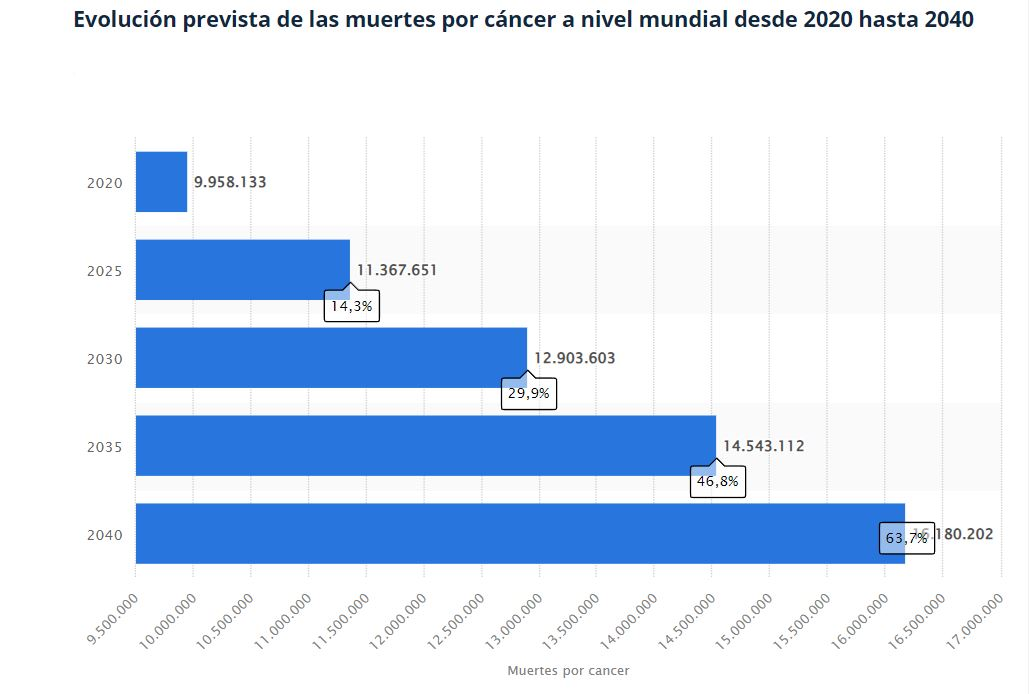
\includegraphics[width=0.75\textwidth]{1/figures/Grafico1DiagnosnitoCancer.JPG}
		\caption{Predicción de número de casos acumulado de cancer a nivel mundial. Fuente: \cite{stadisitc_cancer}}
		\label{1:fig}
	\end{center}
\end{figure}


Sin embargo, una enfermedad que ha afectado durante siglos a la humanidad es el cáncer. Este se caracteriza por su capacidad de alterar el equilibrio de las células del cuerpo humano, provocando un crecimiento anormal y descontrolado de las zonas afectadas a tal grado que puede llegar a invadir otras partes del cuerpo. La Organización mundial de la salud (OMS) afirma que el cáncer es la segunda causa muerte más frecuente en América y una las principales a nivel mundial. En estima que en el año 2022 hubo 20 millones de nuevos casos y 9,7 millones de muertes. Como se pude observar en la figura\ref{1:fig}, según el estudio de Statista publicado en el año 2023 se proyecta que el número de nuevos casos de cáncer crecerá notoriamente en los próximos 20 años.\parencite{OMS_cancer}






Entre los tipos más comunes de cáncer se encuentra el que afecta a la piel el cual se puede contraer a cualquier edad; sin embargo, las personas de mayor riesgo son las que estan expuestos por tiempos prolongados al sol y poseen piel clara. La principal causa es la exposición a la radiación ultravioleta o fuentes artificiales. Según American Cancer Society para el año 2023 morirán aproximadamente que morirán aproximadamente 7,990 personas y aproximadamente aparecerán 97,610 nuevos casos.

Si bien la mayoría de los casos se puede tratar sin complicaciones, existe un porcentaje en el cual puede llegar a ser peligro y potencialmente mortal. Esto principalmente debido a que no es detectado a tiempo o no se cuenta con dermatólogos especializados en esta área.

\begin{figure}[h]
	\begin{center}
		\includegraphics[width=0.5\textwidth]{1/figures/radiación_ultravioleta_peru.png}
		\caption{Pronóstico de radiación UV. Fuente: \cite{SENAMHI_uv}}
		\label{1:fig1}
	\end{center}
\end{figure}



En el caso del Perú, el cáncer de piel está en aumento, especialmente debido a la alta incidencia de radiación ultravioleta (UV) en muchas regiones del país como podemos ver en la figura\ref{1:fig1} el nivel de radiacion ultravioleta el dia 21 de abril del 2024 \parencite{SENAMHI_uv}  y la falta de conciencia sobre la protección solar adecuada. Agregando, la detección temprana y el tratamiento oportuno de esta enfermedad son difíciles por la falta de acceso a servicios de salud especializados en algunas áreas rurales y remotas. Como podemos observar en la siguente figura\ref{1:fig2} La cual nos indica que el 73\%\ de los casos fueron cuando acudieron a un establecimiento de salud en el momento que ya presentaron síntomas muy notorios de cáncer, haciendo evidencia de que el fue diagnosticado de forma tardía. \parencite{cancer_diagnostico}



\begin{figure}[h]
	\begin{center}
		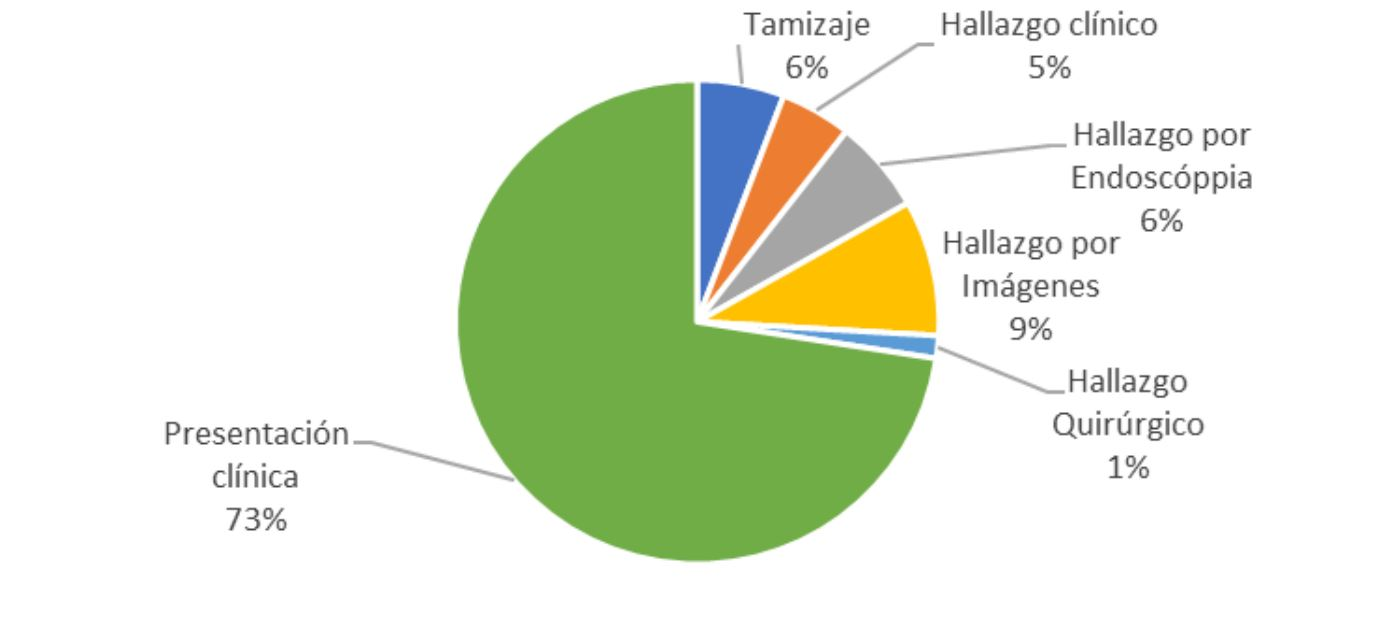
\includegraphics[width=0.8\textwidth]{1/figures/cancer_diagnostico.JPG}
		\caption{Metodo del primer diagnostico DEL CANCER.PERU 2019-2022: \cite{cancer_diagnostico}}
		\label{1:fig2}
	\end{center}
\end{figure}


Aun así, si llegaran a la cita clínica que solicitaron, la probabilidad que esta sea en un ambiente que tenga los recursos necesarios y que sea realizada por un médico dermatólogo especializado en el área, es más seguro que sea considerado como una lesión menor por exposición al sol que sea considerado como un tipo de cáncer de piel. 

Esto principalmente por la complejidad de poder identificarlo, algunas razones son: variedad de tipos de cáncer, estos pueden manifestarse de maneras diferentes en cualquier parte del cuerpo; falta de síntomas, pueden no presentar síntomas o pueden ser similares a los de otras enfermedades menos graves; factores de riesgo, falta del historial del paciente puede hacer que se puedan equivocar en el diagnostico.




\section{Formulación del Problema}

Para realizar la formulación de los problemas del presente trabajo, se elaboró un árbol de problemas (Anexo \ref{1:arbolProblema}).

\subsection{Problema General}
\newcommand{\ProblemaGeneral}{¿Es posible realizar una detección temprana de cáncer de piel en el Perú  haciendo uso de técnicas de Deep Learning y visión por computadora que permita identificar lesiones dermatológicas a partir de imágenes?
}
\ProblemaGeneral
\subsection{Problemas Espec\'{i}ficos}
\newcommand{\Pbone}{
¿Cuáles son los algoritmos de Deep Learning que pueden clasificar con precisión los melanomas y no melanomas entre pacientes peruanos?
}
\newcommand{\Pbtwo}{
¿Cómo evaluar y medir la precisión de los modelos de Deep Learning en la detección de cáncer de piel de tipo melanomas y no melanomas entre pacientes peruanos? 
}
\newcommand{\Pbthree}{
¿Qué tipo de ruido pude haber en las imagenes que dificulté la clasificación de los melanomas y no melanomas entre pacientes peruanos?
}
\newcommand{\Pbfour}{
¿ Qué alternativas se proponen en los trabajos previos para seleccionar características y desarrollar el marco de trabajo de la investigación?
}
\newcommand{\Pbfive}{
¿Cuál es la influencia de las condiciones ambientales y geográficas específicas de Perú en el tratamiento del cáncer de piel?
}

\begin{itemize}
	\item \Pbone
	\item \Pbtwo
	\item \Pbthree
	\item \Pbfour
	\item \Pbfive
\end{itemize}

\section{Objetivos de la Investigación}

Para realizar la formulación de los problemas del presente trabajo, se elaboró un árbol de objetivos (Anexo \ref{1:arbolObjeti}).


\subsection{Objetivo General}
\newcommand{\ObjetivoGeneral}{
Desarrollar un sistema de detección de cáncer de piel mediante el uso de técnicas de Deep Learning y visión por computadora que permita identificar lesiones dermatológicas a partir de imágenes, para realizar una detección temprana.

%%Determinar cuál de las herramientas propuestas en los trabajos previos es la más precisa y confiable en la detección utilizando imágenes dermatoscopias de pacientes peruanos

}
\ObjetivoGeneral
\subsection{Objetivos Espec\'{i}ficos}
\newcommand{\Objone}{
Identificar y comparar los algoritmos de Deep Learning más adecuados para la clasificación de melanomas y no melanomas en imágenes dermatoscópicas de pacientes del Perú.
}
\newcommand{\Objtwo}{
Desarrollar un marco de evaluación que incluya métricas como precisión, sensibilidad, especificidad, valor predictivo positivo(VPP), acurancy y curvas ROC, con la finalidad de evaluar el rendimiento de los modelos de Deep Learning en la detección de melanoma y no melanoma de pacientes del Perú.
}
\newcommand{\Objthree}{
Identificar y evaluar el impacto de estos ruidos en la precisión de la clasificación de melanomas y no melanomas de pacientes del Perú.
}
\newcommand{\Objfour}{
Analizar los diferentes enfoques utilizados en investigaciones anteriores con la finalidad de desarrollar marcos de trabajo efectivos para la clasificación de melanomas y no melanomas de pacientes del Perú.
}
\newcommand{\Objfive}{
Analizar cómo las condiciones ambientales y geográficas pueden afectar los melanomas y no melanomas de pacientes del Perú.
}

\begin{itemize}
	\item {\Objone}
	\item {\Objtwo}
	\item {\Objthree}
	\item {\Objfour}
	\item {\Objfive}
\end{itemize}


\section{Hipótesis}

\subsection{Hipótesis General}
\newcommand{\HipotesisGeneral}{
La aplicación de técnicas de Deep Learning en el análisis de imágenes dermatoscópicas permitirá entrenar un modelo capaz de identificar características específicas asociadas con el cáncer de piel con una precisión igual o superior a la de los dermatólogos especializados, facilitando la detección temprana de esta enfermedad

}
\HipotesisGeneral
\subsection{Hipótesis Específicas}
\newcommand{\Hone}{
	La implementación del algoritmo de Deep Learning adecuado permitirá calcificar con alta precisión los tipos de cáncer de piel melanomas y no melanomas
	
}
\newcommand{\Htwo}{
Realizar un evalución drastica haciedo uso de las métricas nos proporcionara una mejor comprencion de los modelos de Deep Learning en la detección de cáncer de piel melanoma y no melanoma.
	
}
\newcommand{\Hthree}{
	Identificar los tipos de ruidos en las imágenes dermatológicas permitirá tener un modelo con mayor precisión
		
}
\newcommand{\Hfour}{
	Análisis de trabajos previos para el desarrollo de métodos efectivos con la finalidad de mejorar la eficiencia de los modelos.
	
}
\newcommand{\Hfive}{
	Influencia de las condiciones ambientales y geográficas influye en el cáncer de tipo melanomas y no melanomas de pacientes del Perú.
}
\begin{itemize}
	\item \Hone
	\item \Htwo
	\item \Hthree
	\item \Hfour
	\item \Hfive
\end{itemize}

\subsection{Matriz de Consistencia}

Esta fue elavorada para la presente investigación en el cual encontrarn los problemas, objetivos e hipótesis descritas anteriormente en el Anexo \ref{1:table}.

%%Los problemas, objetivos e hipótesis descritas anteriormente se encuentran en la Matriz de Consistencia del Anexo \ref{table}. Además, los objetivos específicos se formularon a partir de una lluvia de ideas luego de examinar los objetivos planteados en los antecedentes, cuyo detalle e item de referencia se encuentra en el Anexo \ref{anexo5}.


%A continuación se presenta la matriz de consistencia elaborada para la presente investigación (véase Anexo \ref{1:table}).


\section{Justificación de la Investigación}

\subsection{Teórica}
Este trabajo de investigación se realiza con la finalidad de apoyar la falta de dermatólogos especialistas en ciertas regiones del Perú.

Haciendo uso de tecinas de Deep Learning en el análisis de imágenes dermatológicas puede predecir si un usuario pueda estar desarrollando cáncer de piel y predecir el tipo. 


\subsection{Práctica}
Existen diversas investigaciones donde se realiza pre-diagnosticos o clasificación de que tipo de cáncer de piel se muestra en la imagen. No obstante, en este caso se trabajará con data etiquetada por dermatólogos peruanos especializados en el área. Esto con la finalidad de tener una mayor precisión en los resultados.

Ademas que se planteara la realización de un prototipo de un sistema que integra el modelo propuesto, el cual funciona en tiempo real capturando la información de las características solamente recibiendo como entrada una imagen de la lesión. 
%%Ademas que se podrá realizar un seguimiento histórico de la lesión, así servirá para ver como evoluciona la lesión. 


\subsection{Metodológica}. 
La implementación de este modelo puede apoyar a los dermatólogos que no tienen tanta experiencia en esta área a realizar un mejor diagnóstico, ya que si se puede detectar a tiempo se puede realizar un tratamiento efectivo. Es importante destacar que esta enfermedad no es mortal; no obstante, existen casos en donde esta enfermedad puede presentar complicaciones. 

Por ello la investigación deberá analizar los resultados para mejorar la capacidad de predicción y la clasificación de los modelos de detección.

\section{Delimitación del Estudio}

\subsection{Espacial}
Para la investigación, se consideraron las investigaciones de distintos países. Sin embargo, los artículos en general se tomaron en cuenta palabras los de idioma inglés. Ademas de solo adquirir los que hacen uso de modelos de machine learning o deep learning.

\subsection{Temporal}
Los datos que serán necesarios para el siguente estudio serán base de datos con imagenes de cáncer de piel(melanoma y no melanoma) las cuales deben estar etiquetadas si son positivas o negativas.
Para la data de entrenamientos se usara un conjunto de datos llamado “Skin Cancer MNIST: HAM10000” del año 2019. Para luego realizar una base de datos con imagenes de pacientes peruanos de una zona específica del Perú.


\subsection{Conceptual}
Esta investigación se enfocará en la implementación de un modelo que logre detectar si una lesión que posees en la piel es un tipo de cancer (melanoma y no melanomas). Para lograrlo, se centrará en el desarrollo y la implementación de un sistema de detección basado en Deep Learning y visión por computadora.


%\chapter{MARCO TEÓRICO}
\section{Antecedentes de la investigación}
En esta sección se presentarán diversos artículos de investigación o tesis las cuales abordarán el tema de la investigación que se tratara, la problematica y las técnicas que se emplearon para afrontar estas. Asimismo, a continuación se presenta un cuadro resumen (véase Anexo \ref{A:table}) de lo que se presenta en esta sección.


%% Tema de investigacion (2)
\subsection{Deep Learning-Based Transfer Learning for Classification of Skin Cancer \citep*{jain2021deep}}
\citeauthor{jain2021deep} realizaron un artículo de investigación el cual fue publicado en la revista «Machine Learning with Applications» en el año 2021. Este fue titulado \citetitle{jain2021deep} la cual traducida al español significa «Aprendizaje por transferencia basado en aprendizaje profundo para la clasificación del cáncer de piela».


\subsubsection{Planteamiento del Problema y objetivo}
El estudio se enfocó en mejorar el diagnóstico temprano del cáncer de piel, que es una de las principales preocupaciones de salud debido a su creciente incidencia. Por ello, el objetivo principal del estudio fue evaluar el rendimiento de diferentes arquitecturas de redes neuronales convolucionales pre-entrenadas. Busacando determinar cuál de estos lograba la mejor precisión en la clasificación


\subsubsection {Metodología empleada por los autores}
\newcommand{\TIDLone}{Recopilación de la data: Se uso un conjunto de datos HAM10000 compuesta por 10015 imágenes dermatoscópicas y siete clases diferentes
}

\newcommand{\TIDLtwo}{ Preprocesamiento: Para evitar los problemas de desequilibrio y duplicados en el conjunto de datos, aplicaron técnicas de aumento de datos.}

\newcommand{\TIDLthree}{Entrenamiento de modelos: Se implementaron diferentes arquitecturas como: VGG19, InceptionV3, InceptionResNetV2, ResNet50, Xception y MobileNet. Ademas que se usaron Adam (Adaptive Moment Estimation) y función de pérdida de Entropía Cruzada Categórica. (Categorical Cross-Entropy Loss) para realizar ajustes de Hiperparámetros.	
}

\begin{itemize}
	\item \TIDLone
	\item \TIDLtwo
	\item \TIDLthree
\end{itemize}


\subsubsection{Resultados obtenidos}
Se concluyó que Xception Net supera al resto de las redes de aprendizaje de transferencia utilizadas en el estudio, con los valores más altos de Accuracy, Avg.Recallm Avg. Precision Av.

\begin{figure}[h]
	\begin{center}
		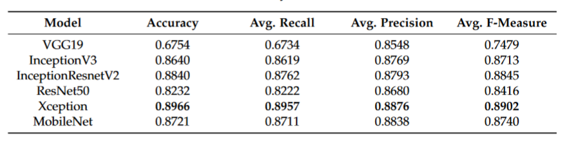
\includegraphics[width=0.8\textwidth]{2/figuras/Deep_Learning_Based_Transfer_Learning_imagen_01.png}
		\caption{Comparación de los resultados de los modelos utilizados. Fuente: \cite{jain2021deep}}
		\label{1:fig 3}
	\end{center}
\end{figure}




\subsection{Classification of Skin Cancer Lesions Using Explainable	Deep Learning \citep*{goceri2023classification}}
\citeauthor{goceri2023classification} realizaron un artículo de investigación el cual fue publicado en el periódico "Sensors" con el número de volumen 22 y página 6915, en el año 2022. Este fue titulado \citetitle{goceri2023classification} la cual traducida al español significa «Clasificación de lesiones de cáncer de piel mediante aprendizaje profundo explicable».

\subsubsection{Planteamiento del Problema y objetivo}

El estudio se enfoca en buscar una solución a las altas tasas de moratalidad del cancer depiel. Por ello se  centran en desarrollar y evaluar modelos de aprendizaje profundo modificados, con la finalidad de mejorar la precisión en la clasificación de lesiones de cáncer de piel como benignas o malignas.




\subsubsection{Metodología empleada por los autores}
\newcommand{\TISCone}{Base de datos: Se uso la bases de datos ISAC2018 Dataset.
}
\newcommand{\TISCtwo}{Preprocesamiento y limpieza de Data: Se aplicaron técnicas para la mejorar de la calidad visual del conjunto de datos, como el estiramiento de contraste, para mejorar la calidad de las imágenes
Luego se empleo la técnica data argumentation para aumentar el número de ejemplos de entrenamiento, lo que incluyó operaciones como rotación, volteo y adición de ruido a las imágenes
	
El conjunto de datos se compone de un total de 3297 imágenes, con 1800 imágenes en la categoría "benigna" y 1497 en la categoría "maligna"
}

\newcommand {\TISCthree} {Modelos de Aprendizaje Profundo: Describen los dos modelos de aprendizaje profundo utilizados en este estudio: MobileNetV2 y DenseNet201. Donde en cada uno de ellos fueron modificados agregando una cierta cantidad de capas convolucionales al final del modelo.
	
}

\newcommand {\TISCfour} {Grad-CAM Visualization: Se emplea para obtener información sobre el aprendizaje de características dentro de los modelos de aprendizaje profundo utilizados en el estudio. Esta técnica proporciona una forma de comprender qué características de la imagen son relevantes para la clasificación realizada por el modelo.}



\begin{itemize}
	\item \TISCone
	\item \TISCtwo
	\item \TISCthree
	\item \TISCfour
	
	
\end{itemize}


\begin{figure}[h]
	\begin{center}
		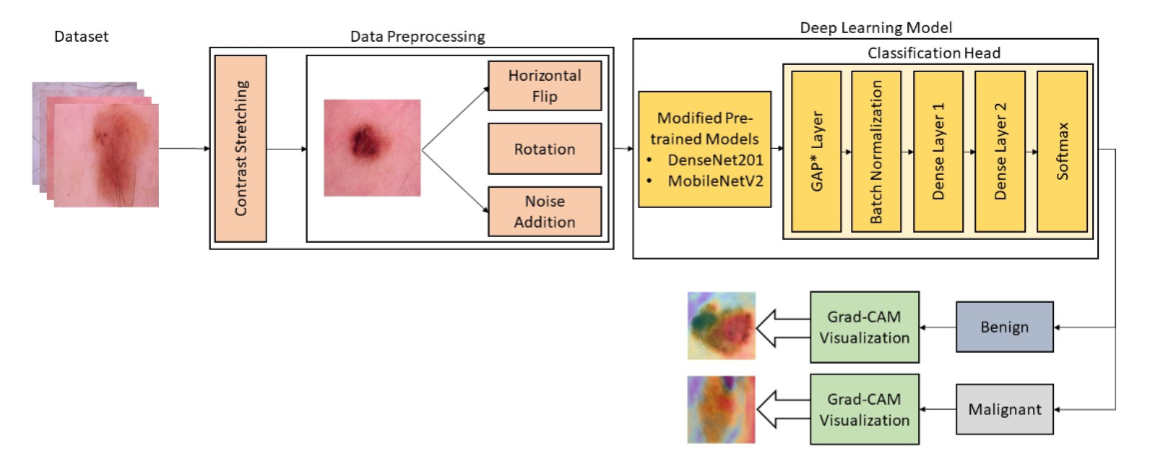
\includegraphics[width=0.8\textwidth]{2/figuras/metodo_ultimo.png}
		\caption{Grafico de la Metodología. Fuente: \cite{goceri2023classification}}
		\label{1:fig 4}
	\end{center}
\end{figure}




\subsubsection{Resultados obtenidos}
Los resultados obtenidos fueron prometedores y demostraron la eficacia de los modelos propuestos.

- El modelo modificado DenseNet201 logró una precisión del 95.50\% en la clasificación de lesiones de cáncer de piel.

- La sensibilidad del modelo fue del 93.96\%

- La especificidad del modelo fue del 97.03\%



\begin{figure}[h]
	\begin{center}
		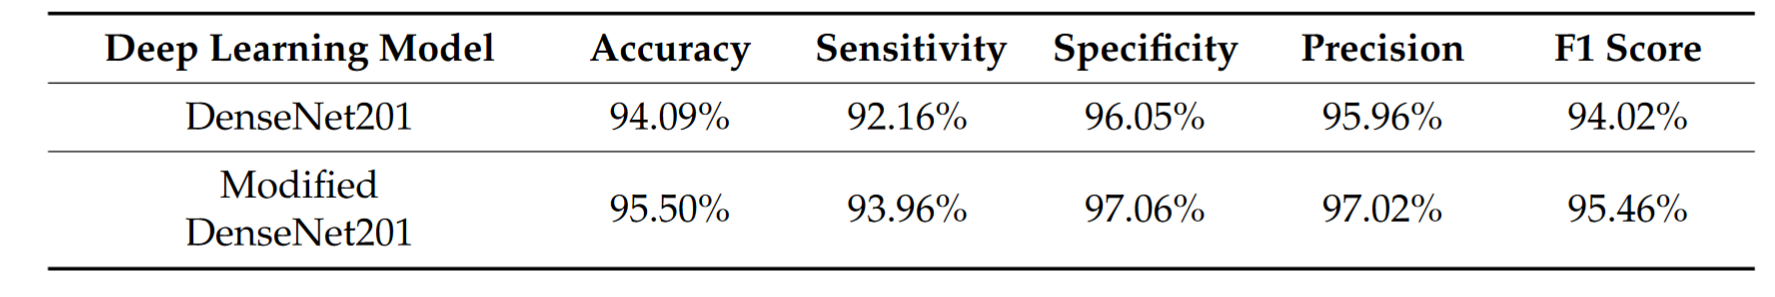
\includegraphics[width=0.8\textwidth]{2/figuras/resultado_ultimo.png}
		\caption{Represación de los 19 estudios. Fuente: \cite{goceri2023classification}}
		\label{1:fig 4}
	\end{center}
\end{figure}



\begin{comment}
	
\subsection{Skin cancer classification via convolutional neural networks: systematic review of studies involving human experts \citep*{haggenmuller2021skin}}
\citeauthor{haggenmuller2021skin} realizaron un artículo de investigación el cual fue publicado en la revista «European Journal of Cancer» en el año 2021. Este fue titulado \citetitle{haggenmuller2021skin} la cual traducida al español significa «Clasificación del cáncer de piel mediante redes neuronales convolucionales: revisión sistemática de estudios en los que participan expertos humanos».

\subsubsection{Planteamiento del Problema y objetivo}
El estudio se enfoca en realizar un análisis de las investigaciones sobre estudios que involucran melanoma y evaluar su posible relevancia clínica mediante tres aspectos principales: características del conjunto de pruebas, prueba entorno y representatividad de los médicos participantes.

\subsubsection{Metodología empleada por los autores}
\newcommand{\TISCone}{Base de datos: Se examinaron los articulos publicados en las siguentes fuentes: PubMed, Medline y ScienceDirect en busca de estudios publicados entre 2017 y 2021.
	
}
\newcommand{\TISCtwo}{Requisitos para entrar a la investigación: Solo se incluían estudios se realizaba comparación directa de los resultados de la IA con médicos y que tenían como objetivo principal una clasificación diagnóstica.
}


\begin{itemize}
	\item \TISCone
	\item \TISCtwo
	%\item \TISCthree
	%\item \TISCfour
	
\end{itemize}

\subsubsection{Resultados obtenidos}
Solo un total de 19 estudios de lectores cumplieron los criterios de inclusión, de los cuales 11 enfoques basados en CNN abordaron la clasificación de imágenes dermatoscópicas, 6 se concentraron en la clasificación de imágenes clínicas, y 2 estudios dermatopatológicos utilizaron imágenes histopatológicas completas digitalizadas.



\begin{figure}[h]
	\begin{center}
		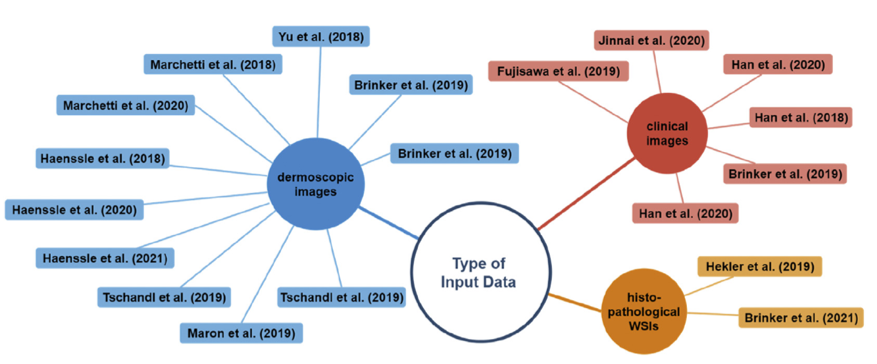
\includegraphics[width=1\textwidth]{2/figuras/Skin_cancer_classification _imagen_01.png}
		\caption{Represación de los 19 estudios. Fuente: \cite{haggenmuller2021skin}}
		\label{1:fig 4}
	\end{center}
\end{figure}

\end{comment}




%% Problematica (2)


\subsection{An enhanced technique of skin cancer classification using deep convolutional neural network with transfer learning models \citep*{ali_2021enhanced}}
\citeauthor{ali_2021enhanced} realizaron un artículo de investigación el cual fue publicado en la revista «Machine Learning with Applications» en el año 2021 publicada por El servier. Este fue titulado \citetitle{ali_2021enhanced} la cual traducida al español significa «Una técnica mejorada de clasificación del cáncer de piel que utiliza una red neuronal convolucional profunda con modelos de aprendizaje por transferencia».

\subsubsection{Planteamiento del Problema y objetivo}
El cáncer de piel es uno de los tipos de cáncer de más rápido crecimiento y que puede causar la muerte, la realización de una detección temprana mejoraría significativamente las posibilidades de supervivencia del paciente. Por ello, el objetivo que se plantea es desarrollar un modelo de clasificación con la finalidad que distinguir las lesiones cutáneas benignas y malignas de forma precisa.


\begin{comment}
\subsubsection{Técnicas empleadas por los autores}
Los autores plantearon emplear diversas técnicas en las diferentes etapas de la metodología. En el caso del procesamiento, se centraron en la transformación de color para mejorar el contraste de la imagen y en un algoritmo de umbralización para detectar y clasificar artefactos de reflexión en las imágenes.

En la extracción de características, utilizaron ResNet50 para extraer características profundas para la clasificación de lesiones de piel.

En la implementación del modelo, emplearon una red neuronal convolucional profunda (DCNN) basada en aprendizaje profundo. Esta red neuronal es especialmente efectiva en tareas de procesamiento de imágenes, siendo capaz de aprender automáticamente características jerárquicas de las imágenes a través de capas convolucionales, lo que la hace ideal para problemas de clasificación de imágenes complejas como en este caso.
\end{comment}

\subsubsection{Metodología empleada por los autores}
\newcommand{\MEone}{ Adquisición de la data: Se uso una base de datos llamada HAM10000 compuesta por 10015 imágenes dermatoscópicas. Donde las imagenes fueron clasificados como malignas o benignas.
}
\newcommand{\MEtwo}{ Preprocesamiento: Se realizo diferentes tecnicas de pre-procesamiento como: reducción de datos, eliminación de burbujas de aire, ruido y artefactos, normalización de los datos y <<data augmentation>> . Esto con la finalidad de mejorar la tasa de clasificación del conjunto de datos en general. 
}

\newcommand{\MEthree}{ Extración de caracteristias: Se realizó una extracción de características para identificar y reconocer patrones en el conjunto de datos. 
}
\newcommand{\MEfour}{Implementación del modelo: Se entreno la red neuronal convolucional profunda (DCNN) y otro grupo de modelos para comprar AlexNet, ResNet, VGG-16, DenseNet, MobileNet.
Se hizo 3 diviciones del conjunto de datos: entrenamiento, validación y prueba de 2 formas distintas.

- 70\% entrenamiento, 20\% validación, 10\% prueba

- 80\% entrenamiento, 10\% validación, 10\% prueba
}



\begin{itemize}
	\item \MEone
	\item \MEtwo
	\item \MEthree
	\item \MEfour

\end{itemize}

\begin{figure}[h]
	\begin{center}
		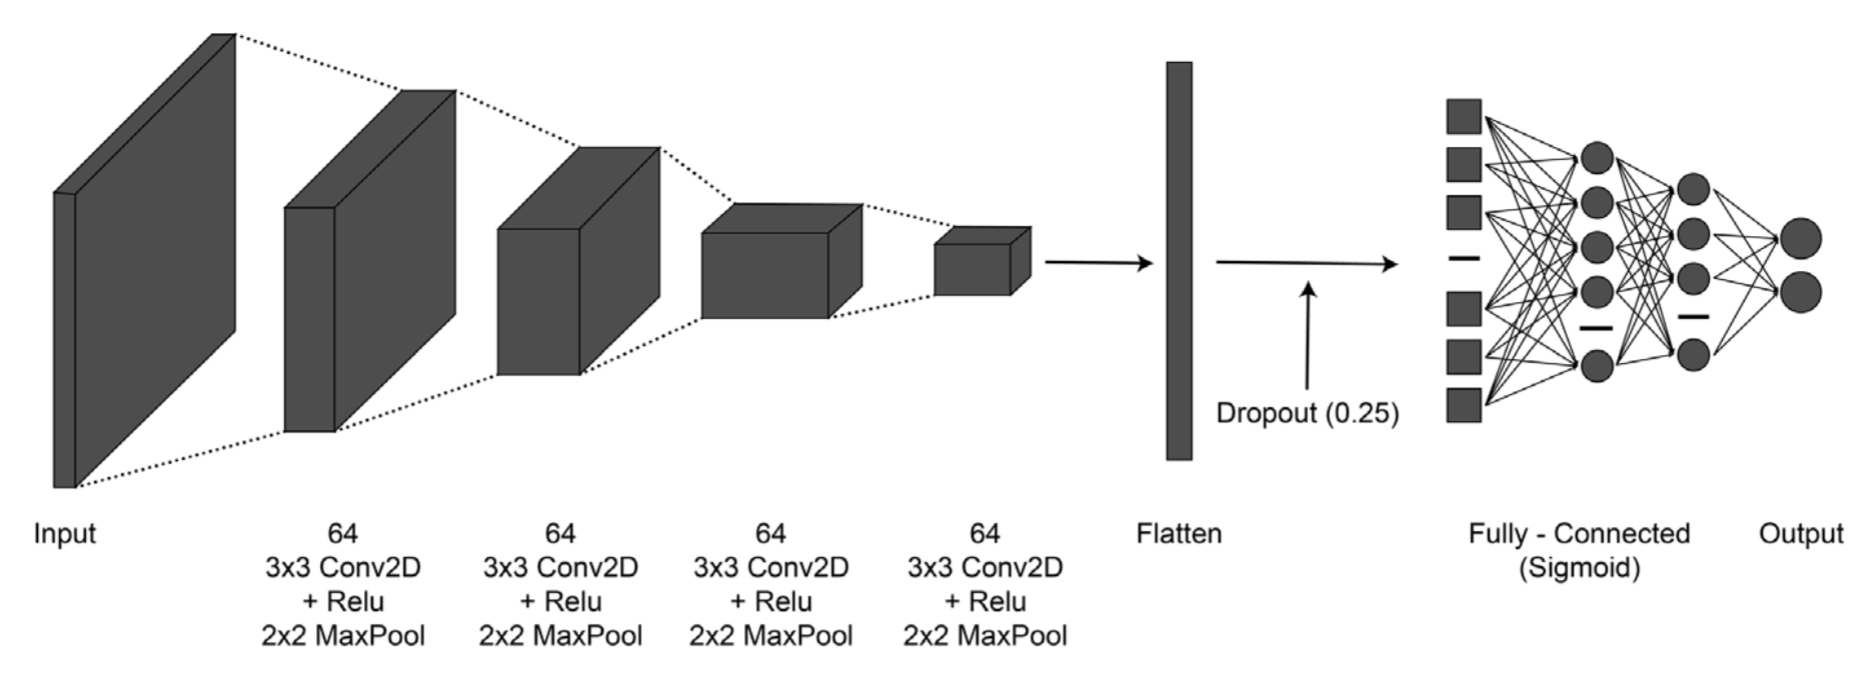
\includegraphics[width=0.8\textwidth]{2/figuras/Problematica_An_enhanced_tecniques_imagen_02.png}
		\caption{Modelo de arquitectura propuesto DCNN .Fuente: \cite{ali_2021enhanced}}
		\label{1:fig 5}
	\end{center}
\end{figure}


\subsubsection{Resultados obtenidos}
Según el articulo el modelo propuesto DCNN fue el que obtuvo una precisión de clasificación del 93.16\% en el conjunto de entrenamiento y 91.93\% en el conjunto de prueba. A comparación del rendimiento que tuvieron los otros modelos de transfer learning como AlexNet, ResNet, VGG-16, DenseNet y MobileNet, los cuales fueron inferiores en términos de precisión, recall, puntaje F1 y tiempo de ejecución.

\begin{figure}[h]
	\begin{center}
		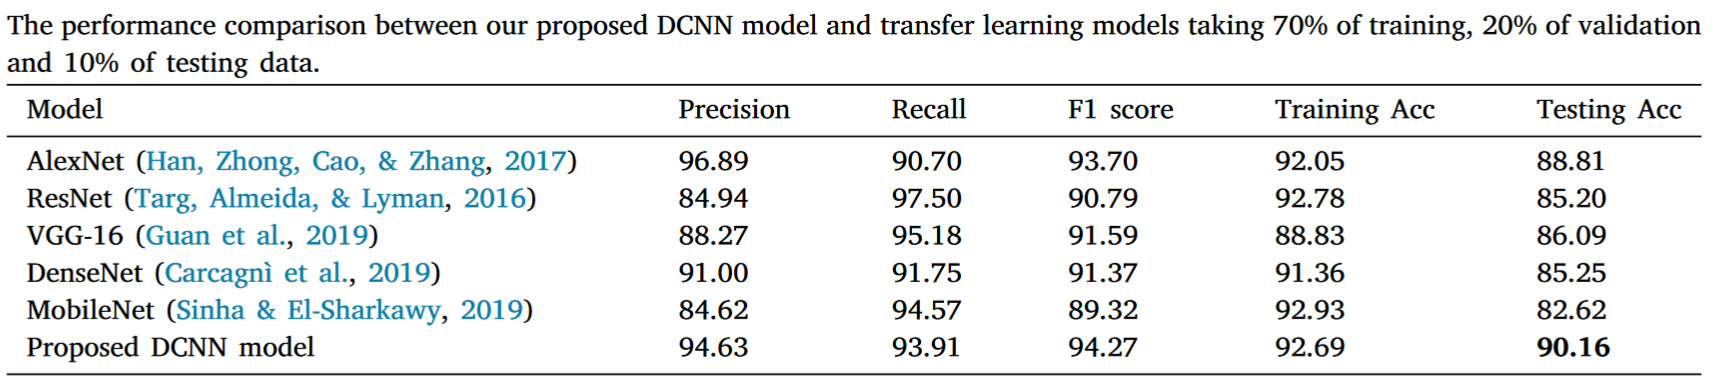
\includegraphics[width=1\textwidth]{2/figuras/Problematica_An_enhanced_tecniques_imagen_01.png}
		\caption{Resultados de modelo DCNN comparandolo con otros modelos Fuente: \cite{ali_2021enhanced}}
		\label{1:fig 6}
	\end{center}
\end{figure}




\subsection{Design of a tool for the classification of skin cancer images using Deep Neural Networks (DNN) \citep*{vargas_2021diseno}}

\citeauthor{vargas_2021diseno} realizaron un artículo de investigación el cual fue publicado en la revista «Ciencia y Tecnología» en el año 2021 publicada por Universidad de Palermo (UP). Este fue titulado \citetitle{vargas_2021diseno}.


\subsubsection{Planteamiento del Problema y objetivo}
Los autores identifican que el cáncer de piel es una enfermedad común a nivel mundial que requiere un diagnóstico temprano para mejorar la calidad de vida de los pacientes. La clasificación automática de lesiones cutáneas presenta un reto debido a su amplia variedad y morfología. Por ende, el objetivo de la investigación es utilizar las ventajas del Deep Learning con la finalidad de desarrollar una red neuronal convolucional (CNN) entrenada para la clasificación de lesiones cutáneas benignas y malignas.


\begin{comment}
\subsubsection{Técnicas empleadas por los autores}
Los autores plantearon emplear diversas técnicas, entre ellas el uso de Data Augmentation para mejorar el tamaño y la calidad de los conjuntos de datos de entrenamiento, lo que ayudó a la construcción de modelos más efectivos.

Posteriormente, realizaron pruebas para ajustar la época, el tamaño del lote y la tasa de aprendizaje, con el fin de establecer valores óptimos y mejorar el rendimiento de los modelos durante el entrenamiento.

Finalmente, utilizaron K-fold Validation y F1 Score para evaluar el rendimiento de los modelos en la clasificación de lesiones benignas y malignas.
\end{comment}


\subsubsection{Metodología empleada por los autores}
\newcommand{\MEDone}{Recopilación de la data: Se uso dos bases de datos entre ellas HAM10000 compuesta por 10015 imágenes dermatoscópicas y ISIC (The International Skin Imaging Collaboration)la cual consta de 2357 imágenes de 226x226 píxeles de enfermedades oncológicas malignas y benignas.
}
\newcommand{\MEDtwo}{ Preprocesamiento:Se aplicó Transfer Learning para compartir características generales de bases de datos extensas, mejorando el rendimient. Haciendo uso de estrategias como Data Augmentation, ajuste de la tasa de aprendizaje y validación K-fold se implementaron para mejorar los modelos.
}

\newcommand{\MEDthree}{ Selección de arquitectura: Evaluaron diferentes arquitecturas como MobileNet V1, MobileNet V2, VGG19, VGG16, Inception V3, ResNet50. 
Al final se seleccionaron MobileNet V1 e Inception V3 como las arquitecturas más adecuadas
}

\newcommand{\MEDfour}{Implementación del modelo: Se implementaron diferentes versiones de modelos, desde el entrenamiento sin congelar capas hasta la adición de capas ocultas y estrategias de regularización. Para evaluar cual es el mejor modelo.
}


\begin{itemize}
	\item \MEDone
	\item \MEDtwo
	\item \MEDthree
	\item \MEDfour
\end{itemize}

\subsubsection{Resultados obtenidos}
El modelo MobileNet V1 alcanzó el mejor rendimiento a comparación de Inception V3. Este con un puntaje F1 del 91.06\%, una sensibilidad del 91.98\% y una tasa de falsos positivos del 9.65\%. 


\begin{figure}[h]
	\begin{center}
		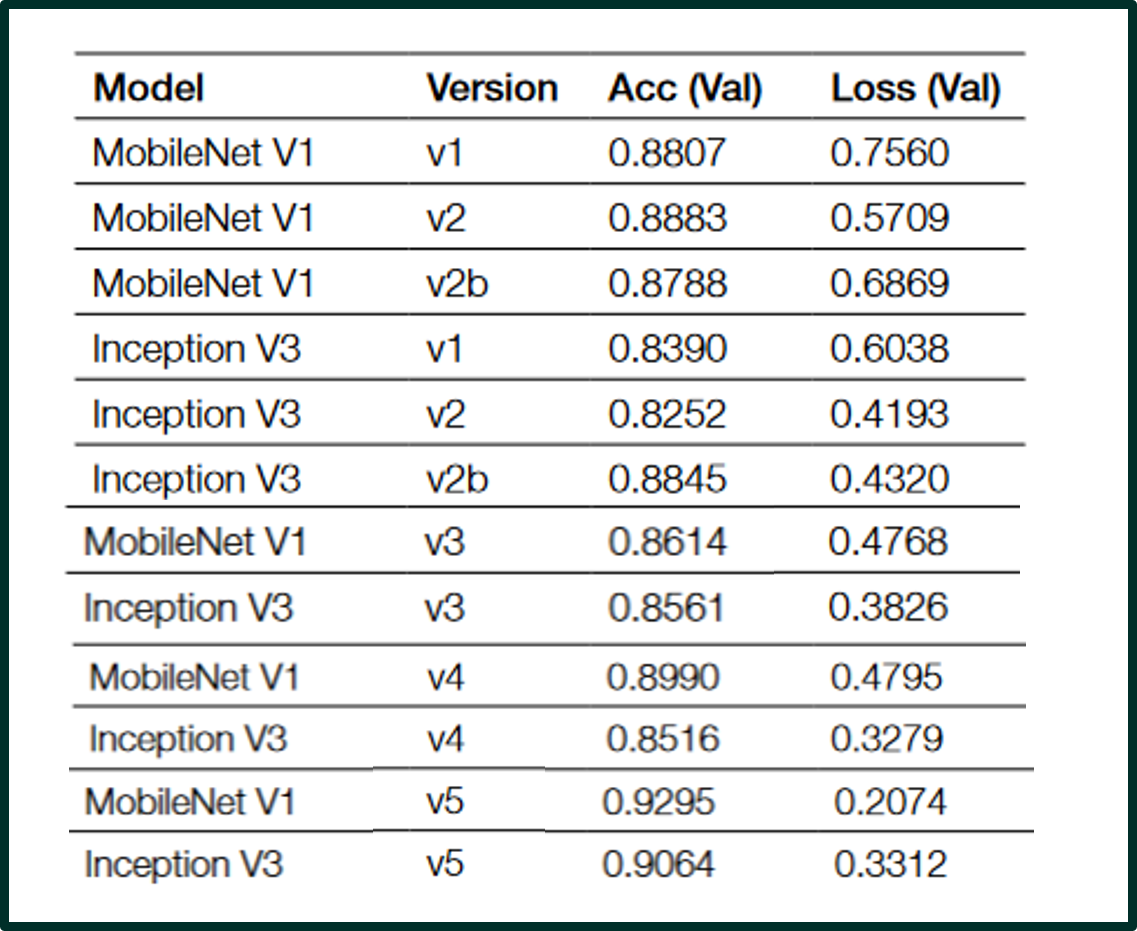
\includegraphics[width=0.6\textwidth]{2/figuras/Design_tool_the_classification_imagen_01.png}
		\caption{Comparacion de los resultados del modelo MobileNet V1 y Inception V3 con diferentes versiones. Fuente: \cite{vargas_2021diseno}}
		\label{1:fig 7}
	\end{center}
\end{figure}




%%% Tecnicas (6)

\subsection{Diagnosis of skin cancer using machine learning techniques \citep*{murugan_2021diagnosis}}

\citeauthor{murugan_2021diagnosis} realizaron un artículo de investigación el cual fue publicado en la revista «Microprocessors and Microsystems» en el año 2021. Este fue titulado \citetitle{murugan_2021diagnosis} la cual traducida al español significa «Diagnóstico del cáncer de piel mediante técnicas de aprendizaje automático».



\subsubsection{Planteamiento del Problema y objetivo}
 El artículo destaca el problema de la detección temprana del cáncer de piel, ya que la piel desempeña un papel vital en el cuerpo humano y cualquier cambio en su funcionamiento puede afectar significativamente la salud general.

Enfocandose que las lesiones cutáneas que son signos clínicos importantes de enfermedades de la piel, como el melanoma y el carcinoma de células basales. Estos son una forma peligrosa de cáncer que puede propagarse rápidamente si no se detecta a tiempo

Por ende, el objetivo principal del estudio es desarrollar un sistema de identificación de enfermedades de la piel basado en imágenes de la piel. Empleando técnicas de aprendizaje automático como SVM, PNN y Random Forest

\begin{comment}
\subsubsection{Técnicas empleadas por los autores}
Según el articulo se realizan comparaciones entre diversas tecnicas para confirmar cual es la mejor.

En el caso la extraccion de caracteristicas: se usaron GLCM, Moment Invariants and GLRLM.

Aquí se presentan algunas de sus ecuaciones:
%%%Ecuacion
\begin{equation}  
	\label{eq:GLCM}
	GLCM = \sum_{x} \sum_{y} (x + a)^p \cdot (y + b)^q \, f(x, y)
\end{equation}


\begin{equation}
		\label{eq:Moment Invariants}
Moment Invariants = \sum_{x=0}^{M-1} \sum_{y=0}^{M-1} x^p \cdot y^q \, f(x, y) \quad \text{para} \quad p, q = 0, 1, 2, 3
\end{equation}


Para comprobar cual modelo obtiene mejores descriptores de las imágenes de lesiones cutáneas. 

Luego, emplearon varios clasificadores de aprendizaje automático: PNN, SVM, Random Forest y SVM + RF (Máquinas de Vectores de Soporte (SVM), Redes Neuronales Probabilísticas (PNN), Bosques Aleatorios (RF) y una combinación de SVM y RF). Para identificar y clasificar diferentes tipos de lesiones de piel.
\end{comment}


\subsubsection{Metodología empleada por los autores}
\newcommand{\MEDSone}{ Recopilación de la data: En este caso no se especifica el tamaño o la fuente exacta del conjunto de datos. Sin embargo, menciona que se empleó un conjunto de datos de imágenes dermoscópicas para identificar y clasificar diferentes tipos de lesiones de piel, como lentigo simple, melanoma, carcinoma basocelular, entre otros.
	
}
\newcommand{\MEDStwo}{ Preprocesamiento: Se dividio en dos etapas: 

- Primera etapa: Removieron el ruido de las imágenes para eliminar pelos y burbujas que pueden afectar la extracción de características,  utilizando un filtro de mediana.

- Segunda etapa: Uso del algoritmo de segmentación Mean Shift para separar la región de interés (ROI) que contiene la lesión del fondo de la imagen.
	
}

\newcommand{\MEDSthree}{ Extracción de características: Uso de tres técnicas para la extracción de características de las imágenes: 
	
- Gray Level Co-Occurrence Matrix (GLCM)

- Moment Invariants(MI)

- Gray Level Run Length Matrix (GLRLM)

}
\newcommand{\MEDSfour}{Implementación del modelo: 
	Se aplican técnicas de clasificación como Máquinas de Vectores de Soporte (SVM), Redes Neuronales Probabilísticas y Bosques Aleatorios, así como la combinación de SVM y Random Forest, con las distintas técnicas para las características extraídas.
}


\begin{itemize}
	\item \MEDSone
	\item \MEDStwo
	\item \MEDSthree
	\item \MEDSfour
\end{itemize}

\begin{figure}[h]
	\begin{center}
		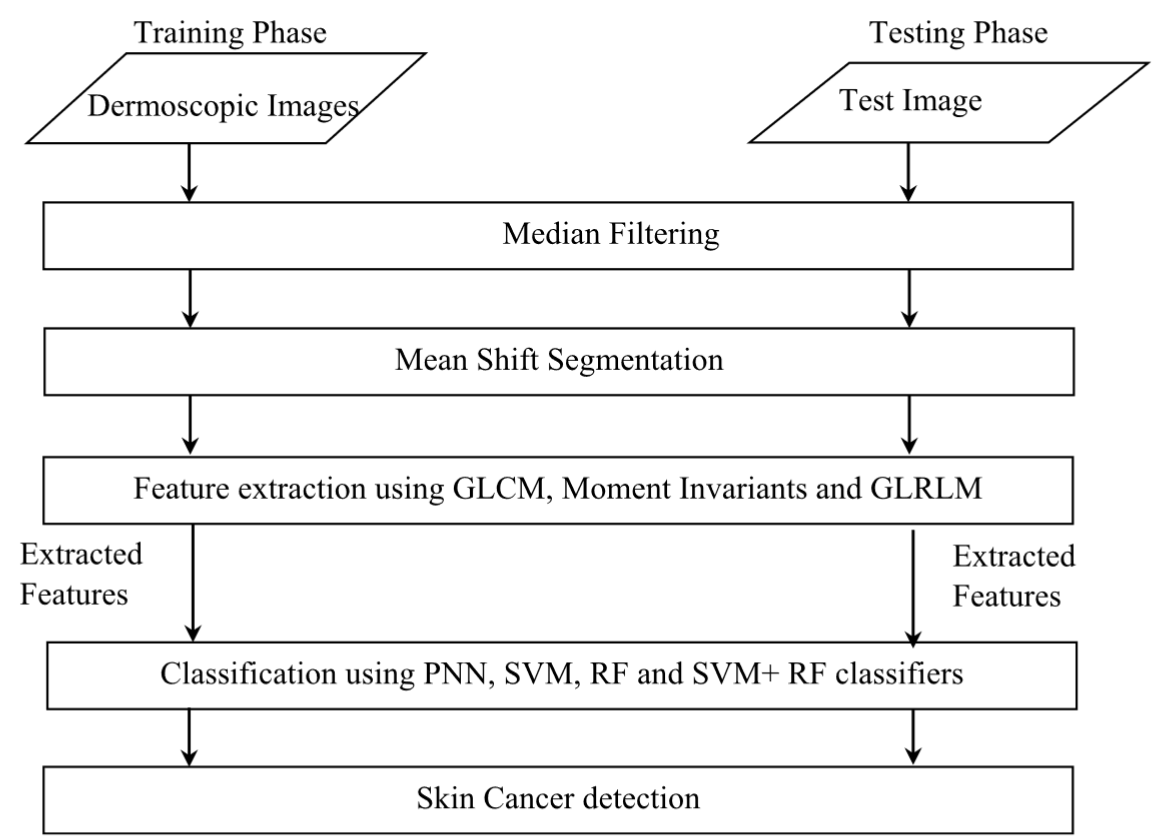
\includegraphics[width=0.6\textwidth]{2/figuras/Tecnica_Diagnosis_skin_cancer_imagen_02.png}
		\caption{Grafica de la Metodología usada . Fuente: \cite{murugan_2021diagnosis}}
		\label{1:fig 8}
	\end{center}
\end{figure}



\subsubsection{Resultados obtenidos}
El rendimiento de los modelos que se emplearon se evaluó en términos de métricas como precisión, sensibilidad y especificidad
Dado como resultado que el mejor clasificador fue la combinación de SVM y Random Forest (SVM+RF) usando un extractor de características GLCM dando un accuracy de 89.31\% 
\begin{figure}[h]
	\begin{center}
		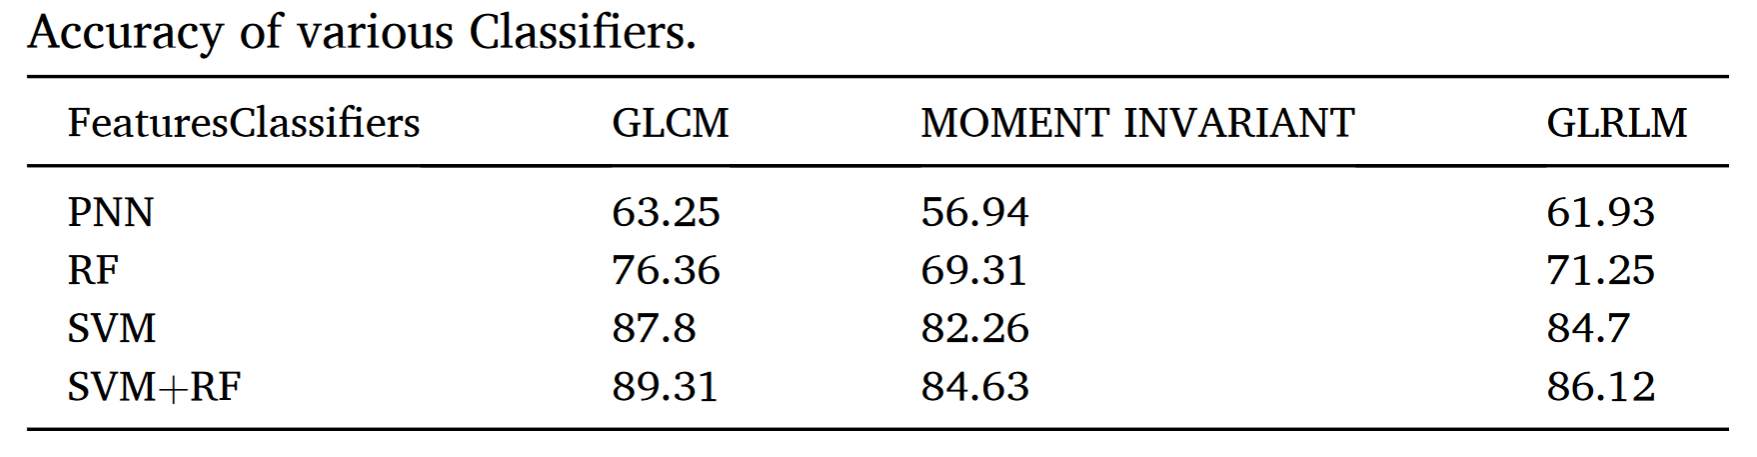
\includegraphics[width=0.75\textwidth]{2/figuras/Tecnica_Diagnosis_skin_cancer_imagen_01.png}
		\caption{Comparación de los modelo empleados con las  tres técnicas para la extracción de características. Fuente: \cite{murugan_2021diagnosis}}
		\label{1:fig 9}
	\end{center}
\end{figure}






\subsection{Multiclass skin cancer classification using EfficientNets – a first step towards preventing skin cancer \citep*{ali_2022multiclass}}
\citeauthor{ali_2022multiclass} realizaron un artículo de investigación el cual fue publicado en la revista «Neuroscience Informatics» en el año 2022. Este fue titulado \citetitle{ali_2022multiclass} la cual traducida al español significa «Clasificación de cáncer de piel multiclase utilizando redes eficientes: un primer paso para prevenir el cáncer de piel».




\subsubsection{Planteamiento del Problema y objetivo}

La clasificación del cáncer de piel presenta una alta dificultad debido a la variabilidad en la apariencia de sus diversas categorías diagnósticas. Aunque los dermatólogos suelen diagnosticar esta enfermedad visualmente, estudios recientes han demostrado que el uso de la  tecnologia pueden superar ayudar a los dermatólogos.

El objetivo principal es desarrollar un sistema de clasificación de cáncer de piel utilizando la técnica de transfer learning en redes neuronales convolucionales pre-entrenadas.

\begin{comment}
\subsubsection{Técnicas empleadas por los autores}
Redes EfficientNets: Se utilizaron los modelos EfficientNets B0-B7 preentrenados con pesos de ImageNet. Estos modelos se ajustaron finamente (fine-tuning) con el conjunto de datos.

Detección de características: Se extrajeron características utilizando redes neuronales convolucionales (CNN) preentrenadas.

Transfer learning: Se aplicó transfer learning para entrenar el conjunto de datos en los pesos preentrenados de ImageNet y ajustar finamente las CNN.

Optimización de hiperparámetros: Se ajustaron hiperparámetros como las tasas de aprendizaje cíclico para entrenar las redes neuronales.

Métricas de evaluación: Se utilizaron métricas como precisión, recall, exactitud y puntaje F1 para evaluar el rendimiento de los modelos. También se emplearon matrices de confusión.
\end{comment}


\subsubsection{Metodología empleada por los autores}

\newcommand{\MEDMone}{Adquisición de la data: Se uso una base de datos llamada HAM10000 compuesta por 10015 imágenes dermatoscópicas. De donde se dibirieron las imagenes en siete difetentes tipos de cancer de piel}

\newcommand{\MEDMtwo}{ Preprocesamiento: Primero se elimino la precencia de elemenotos no relevantes, en este caso los pelos que aparecia en la mayoria de las imagenes. Continuando con la redimencioón de las imagenes de acuerdo con los requerimientos de cada variante de  EfficientNet (B0-B7). Finalizando con el aumento de datos para tener la misma cantidad en cada partición.}

\newcommand{\MEDMthree}{Entrenamiento y validación:
 Los modelos se entrenaron y validaron utilizando técnicas como k-Fold Cross-Validation y se evaluaron con métricas como precisión, recall, exactitud y puntaje F1.}



\begin{itemize}
	\item \MEDMone
	\item \MEDMtwo
	\item \MEDMthree
	
\end{itemize}

\subsubsection{Resultados obtenidos}

Según la tabla de resultados se concluyó que  el modelo EfficientNet B4 logró los mejores resultados con un puntaje F1 del 87\% y una exactitud de clasificación Top-1 del 87.91\%, destacando su eficacia en la clasificación multiclase del cáncer de piel en el conjunto de datos HAM10000.

\begin{figure}[h]
	\begin{center}
		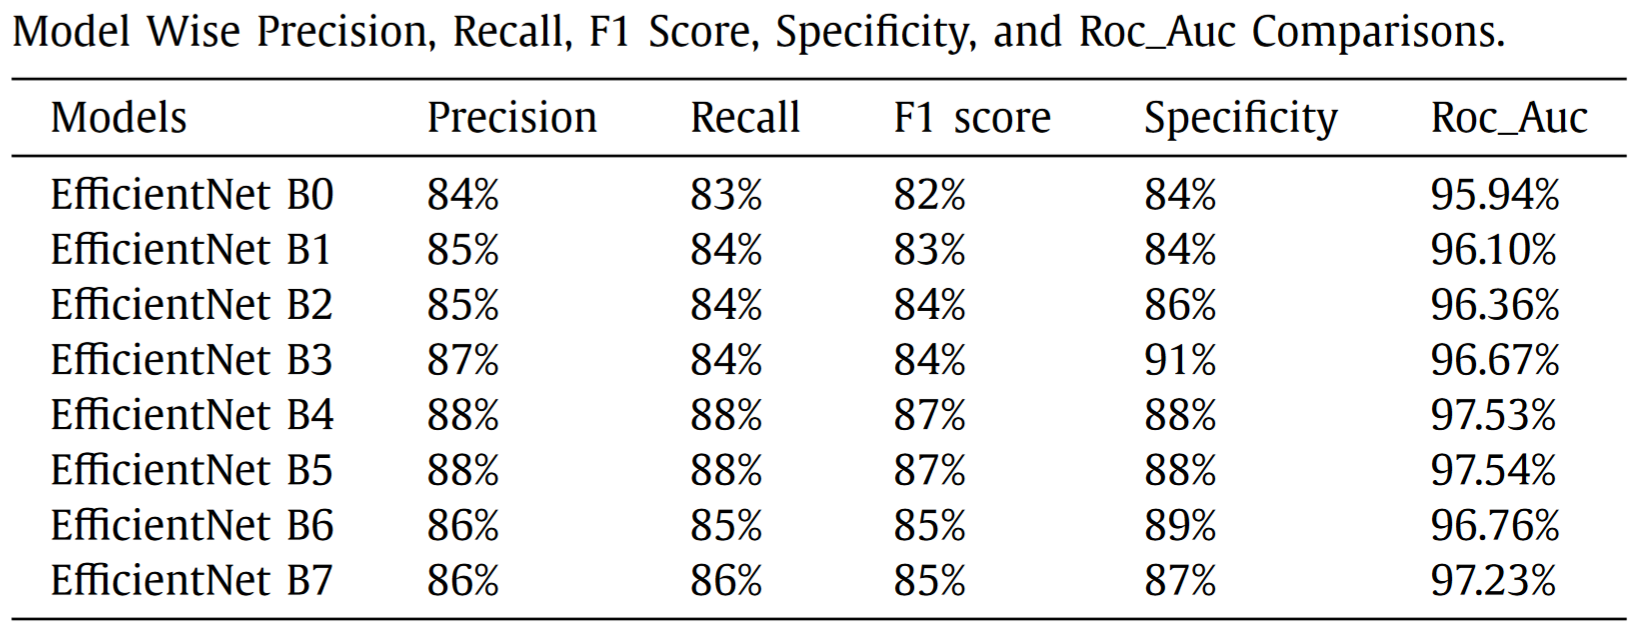
\includegraphics[width=0.8\textwidth]{2/figuras/Multiclass_skin_cancer_imagen_01.png}
		\caption{Comparación de los modelo empleados con las  tres técnicas para la extracción de características. Fuente: \cite{ali_2022multiclass}}
		\label{1:fig 10}
	\end{center}
\end{figure}

\subsection{Skin cancer classification using explainable artificial intelligence on pre-extracted image features \citep*{khater2023skin}}
\citeauthor{khater2023skin} realizaron un artículo de investigación el cual fue publicado en la revista «Intelligent Systems with Applications» en el año 2023. Este fue titulado \citetitle{khater2023skin} la cual traducida al español significa «Clasificación del cáncer de piel utilizando inteligencia artificial explicable en características de imágenes previamente extraídas».

\subsubsection{Planteamiento del Problema y objetivo}
Los autores plantearon la necesidad de desarrollar un modelo de clasificación de cáncer de piel que no solo sea preciso sino también explicativo. Esto usando inteligencia artificial explicativa (XAI) para clasificar lesiones de piel en tres clases: nevus típico, nevus atípico y melanoma


\begin{comment}
\subsubsection{Técnicas empleadas por los autores}
Se emplearon varias técnicas de aprendizaje automático (ML) y de inteligencia artificial explicable (XAI) para clasificar el cáncer de piel, las cuales fueron.

Técnicas de aprendizaje automático (ML): XGBoost, árboles de decisión, random forest y KNN(K-Nearest Neighbors),

Inteligencia artificial explicable (XAI): SHAP (Shapley Additive Explanations), Permutation importance, Partial dependence plot y Local Interpretable Model-agnostic methods(LIME)

\end{comment}

\subsubsection{Metodología empleada por los autores}

\newcommand{\TPSCone}{Recopilación de la data: Se uso un conjunto de datos PH2(recopilación de datos en el departamento de dermatología del Hospital Pedro Hispano)
Este conjunto de datos contiene imágenes dermatoscopia con siete características de entrada y una característica de salida.

}

\newcommand{\TPSCtwo}{ Preprocesamiento: El conjunto de datos se sometio a un proceso de preprocesamiento para mejorar su calidad y preparación para el análisis.}

\newcommand{\TPSCthree}{Extracción de características: Se extrajeron características clave de las imágenes
% Estas características incluyen asimetría, pigment network, dots/globules, streaks, regression areas, blue-white veil regions, y el número de colores presentes en el cáncer de piel.
y usando el método chi-cuadrado se estimo la importancia de cada una de las características y se selecciono las más significativas.
}


\newcommand{\TPSCfour}{ Entrenamiento de modelos de ML: Se entrenaron varios algoritmos de aprendizaje automático (ML) utilizando las características pre-extraídas. Los algoritmos incluyen KNN, XG-boost, árboles de decisión, y bosques aleatorios.
}

\begin{itemize}
	\item \TPSCone
	\item \TPSCtwo
	\item \TPSCthree
	\item \TPSCfour
	
\end{itemize}



\subsubsection{Resultados obtenidos}
El modelo XG-boost como para el Random Forest alcanzó una precisión del min de 94\%. 


\begin{figure}[h]
	\begin{center}
		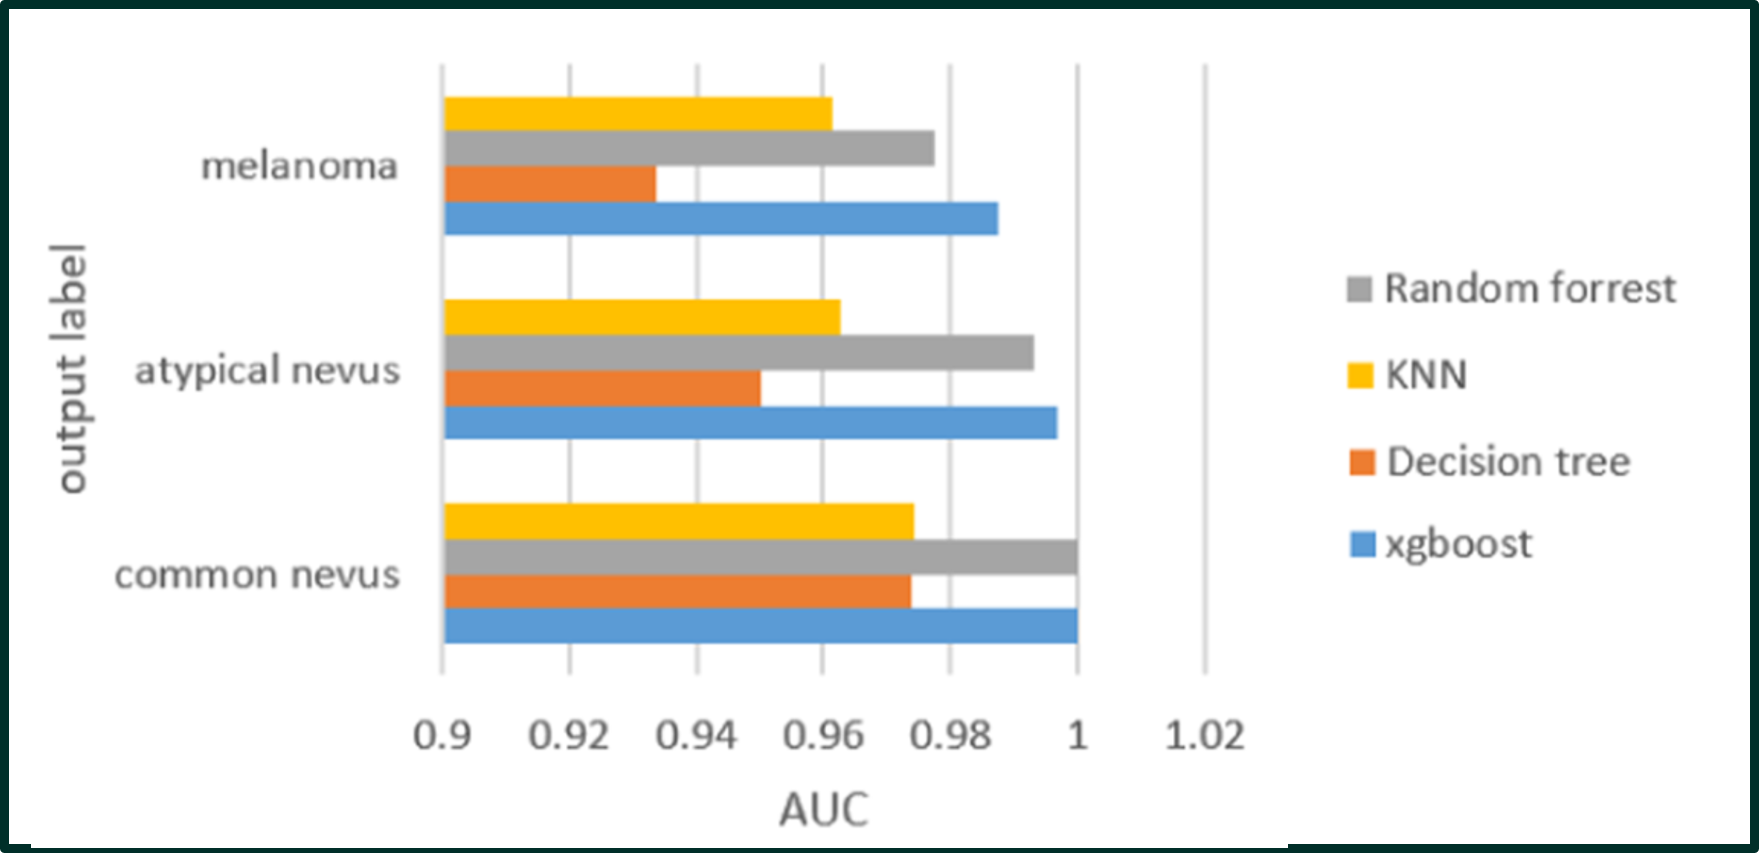
\includegraphics[width=0.6\textwidth]{2/figuras/Skin_cancer_classification_imagen_01.png}
		\caption{Comparación de los modelo empleados con las  tres técnicas para la extracción de características. Fuente: \cite{ali_2022multiclass}}
		\label{1:fig 11}
	\end{center}
\end{figure}





\subsection{An improved transformer network for skin cancer classification \citep*{xin2022improved}}
\citeauthor{xin2022improved} realizaron un artículo de investigación el cual fue publicado en la revista «Computers in Biology and Medicine» en el año 2022. Este fue titulado \citetitle{xin2022improved} la cual traducida al español significa «Una red de transformadores mejorada para la clasificación del cáncer de piel».


\subsubsection{Planteamiento del Problema y objetivo}

El artículo se centra en la necesidad de mejorar la clasificación de imágenes de cáncer de piel para su diagnóstico temprano. Debido al aumento de su incidencia en todo el mundo, lo que representa una gran amenaza para la salud humana. 
En el documento se propone desarrollar un modelo de red transformadora mejorada que pueda lograr una mayor precisión en la clasificación de diferentes tipos de cáncer de piel, mediante el uso de una red neuronal transformadora de visión (VIT).





\subsubsection{Metodología empleada por los autores}
\newcommand{\TPACone}{Recopilación de la data: Se uso un conjunto de datos HAM10000 del archivo ISIC, que incluye siete clases exclusivas de cáncer de piel y recolección de imágenes de cáncer de piel de pacientes hospitalarios mediante dermatoscopia, incluyendo tres tipos de cáncer de piel típicos.	
}

\newcommand{\TPACtwo}{Preprocesamiento: Se llevaron a cabo tres trabajos con la base de datos. Primero, la normalización, para limitar los datos preprocesados a un rango específico y eliminar singularidades y efectos adversos causados por los datos de muestra. Segundo, el aumento de datos, que incluyó técnicas como volteo horizontal y vertical, recorte aleatorio, rotación aleatoria y ajuste de color para mejorar la diversidad de los datos. Por ultimo, el muestreo equilibrado, para garantizar una distribución equitativa de las clases en el conjunto de datos. }

\newcommand{\TPACthree}{Extracción de características: Uso de un transformador de visión multi-escala para dividir una imagen en diferentes tipos de parches. Permitiendo capturar características a múltiples escalas preservando la estructura de los bloques de imagen adyacentes.
}


\newcommand{\TPACfour}{ Entrenamiento de modelos: Se evaluó el modelo propuesto Modelo VIT (Vision Transformer) utilizando métricas como precisión, recuperación, puntaje F1 y AUC en los conjuntos de datos HAM10000 y el conjunto de datos clínico recopilado.
Despues se comparó el rendimiento del modelo propuesto con otros modelos existentes los cuales fueron oft attention network, Ensembles of multi-resolution (EfficientNets), Single model deep learning, Data augmentation for skin classification, Two path CNN model, Deep CNN (Baseline), MobileNetV2, ResNet50, InceptionV2. Con la finalidad de demostrar su eficacia y generalización.	
}

\begin{itemize}
	\item \TPACone
	\item \TPACtwo
	\item \TPACthree
	\item \TPACfour
	
\end{itemize}


\subsubsection{Resultados obtenidos}
El modelo VIT logró un AUC de 0.987, una precisión de 0.941 en el conjunto de datos clínicos recopilados y una precisión de 0.943 en el conjunto de datos HAM10000, superando en 0.3\%, 4.6\%, 1.3\%, 1.2\% y 0.8\% respectivamente a otros modelos.

\begin{figure}[h]
	\begin{center}
		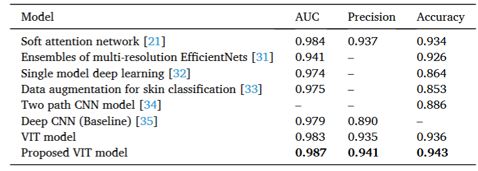
\includegraphics[width=0.9\textwidth]{2/figuras/An_improved_transformer_network _imagen_01.png}
		\caption{Resultados de los Modelo empleados. Fuente: \cite{xin2022improved}}
		\label{1:fig 12}
	\end{center}
\end{figure}




\subsection{Uncertainty quantification in skin cancer classification using three-way decision-based Bayesian deep learning \citep*{abdar2021uncertainty}}
\citeauthor{abdar2021uncertainty} realizaron un artículo de investigación el cual fue publicado en la revista «Computers in Biology and Medicine» en el año 2022. Este fue titulado \citetitle{abdar2021uncertainty} la cual traducida al español significa «Cuantificación de la incertidumbre en la clasificación del cáncer de piel mediante aprendizaje profundo bayesiano de tres vías basado en decisiones».
\subsubsection{Planteamiento del Problema y objetivo}
Los autores se enfocan en la necesidad de cuantificar la incertidumbre en la clasificación de imágenes de cáncer de piel utilizando deep learning, enfocado en la toma de decisiones médicas. Por ello, su objetivo principal es diseñar y validar un nuevo modelo de cuantificación de incertidumbre basado en la teoría de la decisión trinaria y deep learning  para mejorar la confiabilidad y la conciencia de la incertidumbre en la clasificación de imágenes médicas.

\subsubsection{Metodología empleada por los autores}
\newcommand{\TUQSone}{Recopilación de Datos: Los autores recopilaron dos conjuntos de datos de 2 partes: uno de Kaggle y otro del ISIC 2019. Los cuales se realizo un preprocesamiento para preparar las imágenes para su análisis.
}

\newcommand{\TUQStwo}{ Selección de Arquitecturas de Deep Learning: Se seleccionaron cuatro arquitecturas de deep learning conocidas (ResNet152V2, MobileNetV2, DenseNet201 e InceptionResNetV2) como modelos preentrenados en ImageNet. Donde se uso la Optimización Bayesiana (BO) para determinar los mejores valores de hiperparámetros para cada arquitectura y conjunto de datos.
 }

\newcommand{\TUQSthree}{Modelo de tres fases: Se implementó un modelo de tres fases que incluye la detección de muestras inciertas, la clasificación inicial y la clasificación final. Se utilizó un modelo de decisión basado en tres vías (TWDBDL) que combina métodos de incertidumbre con redes neuronales profundas para mejorar la clasificación de cáncer de piel. En la segunda fase, se empleó un modelo de conjunto (EMC) con diferentes arquitecturas de redes neuronales para procesar los datasets
La TWD se utilizó para mejorar la precisión y confiabilidad de las predicciones del modelo al integrarla con las técnicas de cuantificación de incertidumbre en el modelo de aprendizaje profundo.
}

\begin{itemize}
	\item \TUQSone
	\item \TUQStwo
	\item \TUQSthree

\end{itemize}



\subsubsection{Resultados obtenidos}
Para el primer dataset:En la primera fase, el método DE (Deep Ensemble) aplicado a modelos como ResNet152V2, DenseNet201, InceptionResNetV2 y MobileNetV2 logró una precisión del 87.55\%. En la segunda fase, el método EMC (Ensemble Monte Carlo Dropout) obtuvo la mejor AUC, mientras que la precisión de la clase 1 (casos malignos) fue meno

Para el segundo dataset: En la primera fase, el método EMC aplicado a modelos como ResNet152V2, DenseNet201 y DenseNet201 obtuvo una precisión del 89.39\% y un F1-score del 92\%. En la segunda fase, también se utilizó EMC. En la fase final, la precisión de la clase 0 (casos de melanoma) se mantuvo estable, mientras que la precisión de la clase 1 (casos no melanoma) aumentó.

En resumen el modelo TWDBDL propuesto logró buenos resultados de precisión, F1-score y AUC en la clasificación de cáncer de piel, especialmente al detectar y manejar adecuadamente las muestras inciertas.

\begin{figure}[h]
	\begin{center}
		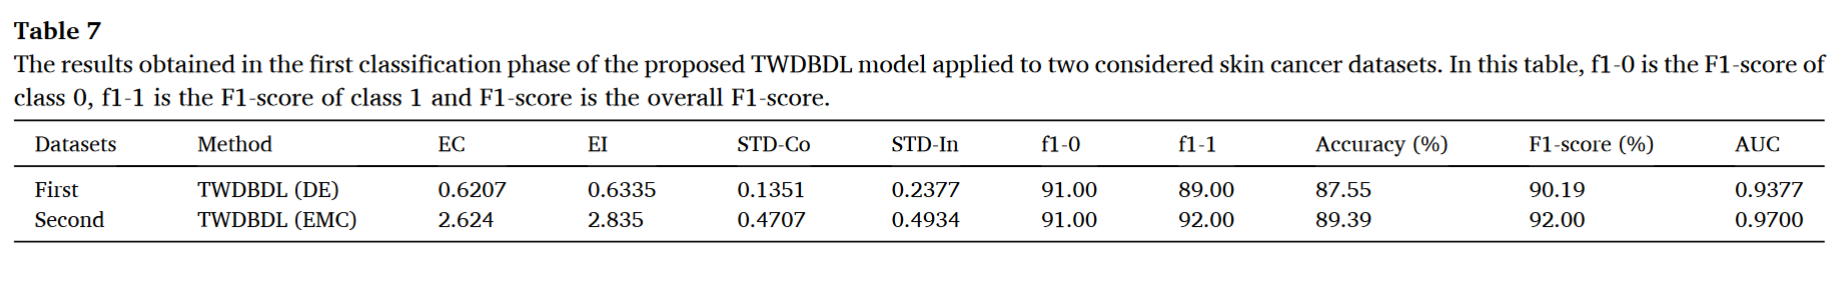
\includegraphics[width=1\textwidth]{2/figuras/Uncertainty_quantification_skin _imagen_01.png}
		\caption{Resultados de los Modelo empleados. Fuente: \cite{abdar2021uncertainty}}
		\label{1:fig 13}
	\end{center}
\end{figure}


\subsection{A multi-class skin Cancer classification using deep convolutional neural networks \citep*{chaturvedi2020multi}}
\citeauthor{chaturvedi2020multi} realizaron un artículo de investigación el cual fue publicado en «Springer Science+Business Media, LLC, part of Springer Nature 2020» en el año 2020. Este fue titulado \citetitle{chaturvedi2020multi} la cual traducida al español significa «Una clasificación de cáncer de piel de múltiples clases utilizando redes neuronales convolucionales profundasl».

\subsubsection{Planteamiento del Problema y objetivo}


El estudio se enfoca en relaizar una clasificación precisa de diferentes tipos de cáncer de piel utilizando técnicas de aprendizaje profundo, ya que se requiere un diagnóstico temprano y preciso para asegurar un tratamiento efectivo para los pacientes. 
Por ello, la investigación, busca desarrollar un sistema basado en aprendizaje profundo que clasifique múltiples clases de cáncer de piel con alta precisión, apoyando la mejorar, eficiencia y precisión del diagnóstico, lo que en última instancia resultará en una atención médica superior para los pacientes con cáncer de piel. 
 
 %Esta innovación promete transformar el proceso diagnóstico, haciéndolo más rápido y uniforme.






\subsubsection{Metodología empleada por los autores}
\newcommand{\TUAMCone}{Recopilación de la data: Se uso los siguetes conjustos de datos: ISIC2017, ISIC2018, y HAM10000. Donde se realizó ajustes para asegurar que los datos estén en un formato adecuado para el entrenamiento de los modelos.
}

\newcommand{\TUAMCtwo}{Implementación de Modelos: Se utilizan diferentes arquitecturas de redes neuronales convolucionales profundas como Xception, InceptionV3, ResNetXt101, InceptionResNetV2 y NASNetLarge para la clasificación de siete tipos de cáncer de piel. }

\newcommand{\TUAMCthree}{Optimización de Modelos(hiperparametos): Se emplean optimizadores como stochastic gradient descent with momentum (SGDM) y adaptive moment estimation (Adam) para ajustar los modelos y minimizar la función de pérdida.
}


\newcommand{\TUAMCfour}{Evaluación de Desempeño: Se evalúa el desempeño de los modelos en un conjunto de validación de 1103 imágenes, calculando métricas como recall, precision, exactitud (accuracy) y F1-score para cada modelo y para las combinaciones de modelos de ensemble.
	
}

\begin{itemize}
	\item \TUAMCone
	\item \TUAMCtwo
	\item \TUAMCthree
	\item \TUAMCfour
\end{itemize}

\subsubsection{Resultados obtenidos}

El accuracy más alto se logró con el modelo ResNeXt101 y InceptionResNetV2, en ambos casos con un 93.20%.
No obstante ResNeXt101 consiguio una mejor precisión que InceptionResNetV2 por una diferencia de 1\%.

\begin{figure}[h]
	\begin{center}
		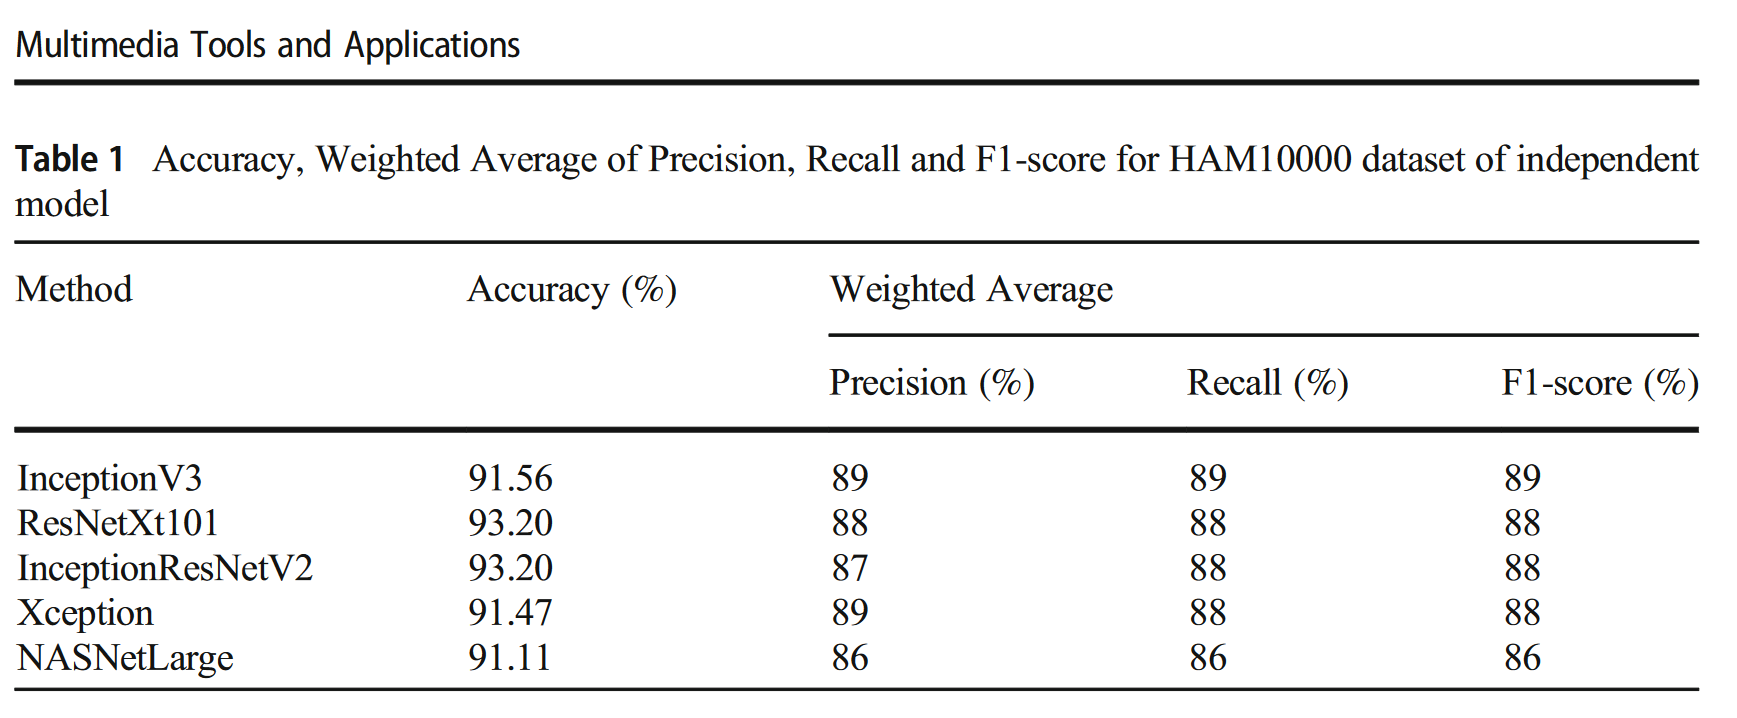
\includegraphics[width=0.8\textwidth]{2/figuras/An_improved_network_skin_cancer_classification_imagen_01.png}
		\caption{Resultados de los Modelo empleados. Fuente: \cite{chaturvedi2020multi}}
		\label{1:fig 14}
	\end{center}
\end{figure}







\section{Bases Teóricas}
%% Vaaraible independiente Deep Learning Visión por computadora


\subsection{Inteligencia Artificial}
La inteligencia artificial (IA) se enfoca en crear sistemas y programas capaces de realizar tareas de la misma manera que lo haría un ser humano. Estos sistemas están diseñados para adaptarse y mejorar con la experiencia, reconocer patrones, tomar decisiones y aprender de datos. 

El termino Inteligencia Artificial fue dado a conocer en el año 1956 durante la Conferencia Dartmouth en Hanover, Nuevo Hampshire (Estados Unidos), donde se propuso la posibilidad de crear una máquina que pudiera pensar como un ser humano.  No obstante, esta a estado presente mucho antes desde de trabajos de investigación, hasta en el cine y novelas representando como ciencia ficción. 
Actualmente, se ha convertido en una de las tecnologías revolucionarias y de mayor interés de investigación.


\begin{figure}[h]
	\begin{center}
		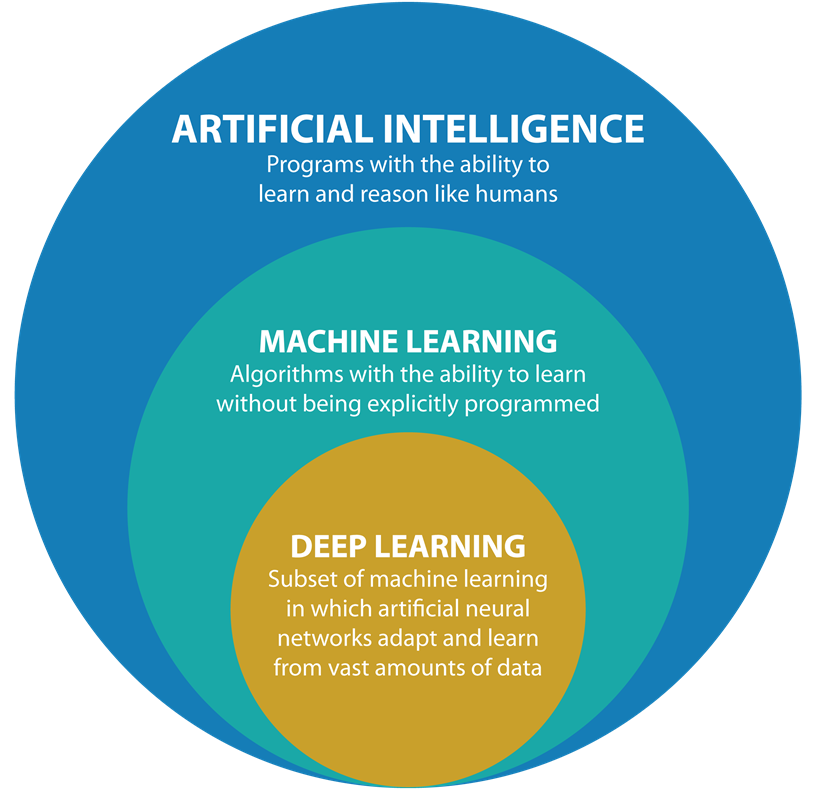
\includegraphics[width=0.5\textwidth]{2/figuras/imagenes/IA_ML_DL.png}
		\caption{Grafico de IA. Fuente: \cite{IA_}}
		\label{1:fig 16}
	\end{center}
\end{figure}

\subsection{Features Vectors}
Un vector de características, es una representación numérica de un objeto, instancia o dato en un espacio multidimensional, donde cada dimensión del vector corresponde a una característica particular del objeto. Estos vectores se utilizan en una variedad de campos, especialmente en el Machine Learning(ML) y Deep Learning(DL), para hacer predicciones y entrenar modelos.

Son cruciales porque pueden capturar de manera efectiva las propiedades pertinentes de los datos, lo que facilita el aprendizaje de los modelos y mejora su rendimiento predictivo. Un buen diseño puede aumentar la velocidad de entrenamiento y reducir la complejidad de los problemas.


\subsubsection{GLCM (Gray Level Co-occurrence Matrix)}

La Matriz de Co-ocurrencia de Niveles de Gris (GLCM), también denominada matriz de dependencia espacial de escala de gris, es una herramienta utilizada en el campo de la visión por computadora y el procesamiento de imágenes para analizar la textura de una imagen. Este captura la relación espacial entre los píxeles en una imagen al cuantificar la frecuencia con la que pares de valores de intensidad de píxeles ocurren juntos en diferentes direcciones y distancias. Este método estadístico para analizar la textura toma en cuenta la relación espacial de los píxeles, creando una GLCM y extrayendo medidas estadísticas de esta matriz. Las funciones de GLCM caracterizan la textura de una imagen calculando con qué frecuencia los pares de píxeles que muestran valores específicos y se encuentran en una relación espacial concreta ocurren en una imagen. Una vez creadas las GLCM usando graycomatrix, se pueden derivar varias estadísticas de ellas empleando graycoprops, proporcionando información detallada sobre la textura de la imagen.
\parencite{mathworksAnxE1lisisTextura}

\subsubsection{Moment Invariant}

Los Momentos Invariantes son características numéricas de una distribución de píxeles en una imagen que son invariantes a transformaciones geométricas como traslación, rotación y escala. Estos momentos, calculados a partir de los valores de intensidad de los píxeles, estos momentos proporcionan información sobre la forma y la distribución de los objetos en la imagen. Se utilizan en aplicaciones como el reconocimiento de formas, describiendo la forma de objetos en imágenes para identificar y reconocer patrones independientemente de su orientación o tamaño, y en la detección de objetos, donde sirven como características para detectar objetos en imágenes basándose en su forma y estructura.


\subsubsection{GLRLM (Gray Level Run Length Matrix)}
La Matriz de Longitud de Corrida de Niveles de Gris (GLRLM) es una técnica utilizada para analizar la textura de una imagen midiendo la longitud y la frecuencia de regiones contiguas con el mismo nivel de gris en diferentes direcciones. Esta técnica describe cuántas veces aparecen píxeles con un cierto nivel de gris en una imagen a lo largo de una dirección específica, proporcionando información sobre la homogeneidad y la textura de la imagen. La GLRLM se calcula para diferentes direcciones, generalmente 13 en 3D o 4 en 2D, y para cada nivel de gris, la matriz contiene la cantidad de veces que aparece una secuencia continua de píxeles con ese nivel de gris en una dirección específica.

Se utiliza en diversas aplicaciones, como el análisis de imágenes médicas, el procesamiento de imágenes industriales, la segmentación de texturas y el reconocimiento facial. La GLRLM permite extraer características de textura como la longitud promedio de carrera, la intensidad promedio y la homogeneidad, y ayuda a identificar regiones inusuales o anómalas en una imagen al detectar patrones de textura distintivos.


\subsection{Aprendizaje Automático  (Maching Learning)}
Es un subcampo de la inteligencia artificial que se centra en el desarrollo de algoritmos y modelos. Permitiendo a las computadoras aprender a partir de datos ya etiquetados y tomar decisiones según la información brindada, esto identificando patrones en los datos y utilizando estos para hacer predicciones o tomar decisiones.
Este tiende a aplicarse en los siguientes temas: detección de fraudes, predicciones, clasificación, sistemas de recomendación.
Este aprendizaje requiere datos de entrenamiento para que funcionen, ademas de mayormente trabajar con data estructurada.

\subsubsection{K-Nearest Neighbors (KNN)}
El algoritmo de K-Nearest Neighbors (KNN) es un método de aprendizaje supervisado utilizado tanto para problemas de clasificación como de regresión. Funciona asignando una etiqueta de clase a un punto de datos basándose en la mayoría de las etiquetas de clase de sus vecinos más cercanos en el espacio de características. En otras palabras, clasifica un punto de datos basándose en las clases de los puntos que están más cerca de él en el espacio de características.

El funcionamiento del algoritmo KNN es relativamente simple: dado un nuevo punto de datos, el algoritmo calcula la distancia entre ese punto y todos los demás puntos de datos en el conjunto de entrenamiento. Luego, selecciona los K puntos más cercanos (vecinos) al nuevo punto y determina la clase mayoritaria entre estos vecinos. Esa clase mayoritaria se asigna al nuevo punto de datos como su etiqueta de clase. La elección del valor de K es crítica y puede afectar significativamente el rendimiento del algoritmo: valores más pequeños de K pueden hacer que el modelo sea más susceptible al ruido, mientras que valores más grandes de K pueden dar como resultado fronteras de decisión más suaves pero también pueden disminuir la precisión del modelo. KNN es un algoritmo simple pero poderoso, especialmente para conjuntos de datos pequeños o cuando no se asume una estructura particular en los datos. Sin embargo, su eficacia puede verse limitada en conjuntos de datos con muchas características o cuando los datos están altamente dimensionales.


%\subsubsection{Random Forest (RF)}

%\subsubsection{Decision Tree}

%\subsubsection{XGBoost}

%\subsubsection{Probabilistic Neural Network (PNN)}

\subsection{Aprendizaje Profundo (Deep Learning)}
Es un subcampo del aprendizaje automático que utiliza redes neuronales artificiales con múltiples capas (profundas) para modelar y resolver problemas complejos. Las redes neuronales profundas se caracterisan por la necesidad de recibir grandes conjuntos de datos estos pueden ser estructurados o no estructurado. Con la finalidad de aprender representaciones jerárquicas de los datos, lo que permite la automatización de la extracción de características.

Este tiende a aplicarse en los siguientes temas: Reconocimiento de voz y visión por computadora, procesamiento de lenguaje natural (NLP), Diagnóstico médico, conducción autónoma, entre otros.

%\subsubsection{EfficientNets}

\subsubsection{Deep Neural Networks (DNN)}
Son modelos de aprendizaje automático que se destacan por su estructura de múltiples capas de neuronas, permitiendo aprender representaciones complejas de los datos. Estas redes están diseñadas para realizar un aprendizaje jerárquico, donde las primeras capas aprenden características simples de los datos de entrada, mientras que las capas posteriores combinan estas características para formar representaciones más abstractas y sofisticadas.

El funcionamiento implica procesar los datos de entrada a través de varias capas de neuronas y ajustar los pesos de la red iterablemente mediante retropropagación del error para reducir las diferencias entre los resultados reales y las predicciones del modelo. Este método de aprendizaje profundo ha demostrado un gran éxito en una variedad de campos, como la robótica, el procesamiento de lenguaje natural y la visión por computadora, ofreciendo soluciones poderosas y automatizadas para una amplia gama de problemas de análisis de datos y toma de decisiones.




%\subsubsection{Deep Convolutional Neural Network (DCNN)}




\subsection{Computer Vision}
Se centra en entrenar a las máquinas para que interpreten las imágenes o videos de manera similar a como lo hacen los humanos. Esto implica la adquisición, el procesamiento, el análisis y la comprensión de imágenes y datos visuales para automatizar tareas que requieren la visión humana.
Algunas tecnologías y algoritmos en esta área son:
\newcommand{\CVone}{ Comparación estadística: Los algoritmos son capaces de  realizar comparaciones y análisis detallados de los objetos, más allá de ubicarlos en un plano.}
\newcommand{\CVtwo}{Detección de objetos: Los algoritmos son capaces de localizar y claisficar varios objetos en una imagen o en videos. Algunos algoritmos son YOLO (You Only Look Once), SSD (Single Shot MultiBox Detector), Faster R-CNN }
\newcommand{\CVthree}{ Análisis de Movimiento: Capacidad de seguir el movimiento y la dirección de un objetos o personas en una secuencia de video. Ejemplos: Optical Flow, Tracking algorithms (Kalman Filter, Mean-Shift, etc.). }

\begin{itemize}
	\item \CVone
	\item \CVtwo
	\item \CVthree
\end{itemize}


\section{Marco Conceptual}
%Varaibl dependiente Diagnostico de cancer

\subsection{El Cáncer}
Según la página del Instituto nacional del cáncer esta enfermedad se caracteriza por la multiplicación de algunas células anormales o dañadas del cuerpo humano, que se dispersan a otras partes del organismo. Llegando a formar tumores. \parencite{cancer_2024 }
El origen de este puede atribuirse a errores en la división celular, factores hereditarios o influencias externas como el entorno y la exposición a sustancias químicas. El desarrollo del cáncer es único en cada individuo, ya que cada persona tiene combinaciones genéticas diferentes, lo que hace que el tratamiento no sea igual para todos los casos.

\begin{figure}[h]
	\begin{center}
		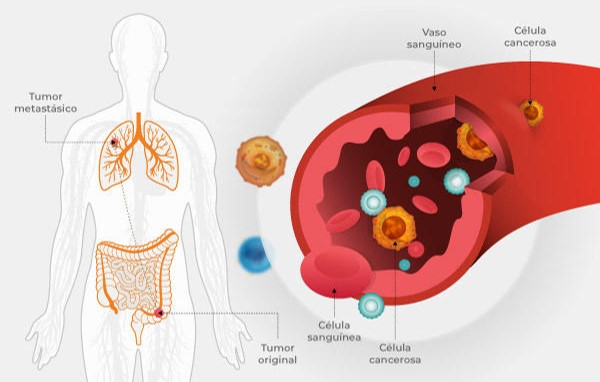
\includegraphics[width=0.6\textwidth]{2/figuras/imagenes/queeselcancer.jpg}
		\caption{Ejemplo como el cancer se traslada a otras partes del cuerpo. Fuente: \cite{cancer_2024}}
		\label{1:fig 15}
	\end{center}
\end{figure}


\subsection{Cáncer de Piel}
El cáncer de piel es el tipo de cáncer más prevalente a nivel mundial. Si bien algunas personas presentan un riesgo de contraerlo, puede afectar a cualquier persona. Este se origina a partir de la formación de células malignas en el tejido cutáneo.
Suele desarrollarse en áreas de la piel que están expuestas al sol; sin embargo, también puede aparecer en zonas que normalmente no están expuestas a la luz solar.
Las principales causas del cáncer de piel se deben a la exposición excesiva a los rayos UV del sol, así como al uso de camas bronceadoras y lámparas solares. Los rayos UV tienen la capacidad de dañar las células de la piel. A corto plazo, este daño puede resultar en quemaduras solares. Con el tiempo, la acumulación del daño por rayos UV provoca cambios en la textura de la piel, envejecimiento prematuro y, en ocasiones, cáncer de piel. \parencite{cancer_piel_clinic_2024}

\subsection{Sintomas del Cáncer de Piel}
Según la American Cancer Society, los médicos sugieren que los exámenes de la piel se incluyan en las revisiones médicas de rutina. De lo contrario, recomiendan que las personas examinen su propia piel aproximadamente una vez al mes. Este autoexamen debe realizarse frente a un espejo, en una habitación bien iluminada, para poder revisar cada área del cuerpo hasta las difíciles de ver. Es importante tener en cuenta la regla del "ABCDE" para identificar signos comunes de problemas en la piel: Asimetría, Borde, Color, Diámetro y Evolución. Estas pautas ayudan a detectar posibles irregularidades en la piel que podrían indicar la presencia de cáncer u otras afecciones.
\parencite{information_cancer}

%\subsection{Factores de Riesgo}



\subsection{Tipos del Cáncer de Piel}
El cáncer de piel se clasifica en dos grandes categorías: cáncer de piel de tipo no melanoma y cáncer de piel de tipo melanoma. El cáncer de piel de tipo no melanoma se subdivide en carcinomas de células basales y carcinomas de células escamosas. Aunque generalmente son malignos, pueden curarse; sin embargo, si no se tratan a tiempo, pueden causar desfiguración y resultar muy costosos de tratar. Por otro lado, el cáncer de piel de tipo melanoma es responsable de la mayoría de las muertes relacionadas con el cáncer de piel, debido a su tendencia a propagarse a otras partes del cuerpo, incluidos los órganos vitales.

\subsection{Melanoma}
El melanoma, también conocido como melanoma maligno y melanoma cutáneo, se origina a partir de los melanocitos, las células especializadas de la piel encargadas de producir melanina. La melanina es responsable del tono bronceado o rojizo que adquiere la piel al exponerse al sol. Este tipo de cáncer tiene un gran potencial maligno, siendo responsable de más del 90\% de las muertes relacionadas con el cáncer de piel. Aunque el melanoma afecta principalmente a la piel, también puede desarrollarse en las mucosas y dentro del ojo. Generalmente, los melanomas se forman en la piel sana, pero en aproximadamente un 20-30\% de los casos, pueden desarrollarse sobre un lunar preexistente.  \parencite{cancer_tipo_melanoma}
Este comportamiento agresivo y su capacidad de propagarse rápidamente a otras partes del cuerpo, incluidos los órganos vitales, hacen que el melanoma sea especialmente peligroso y mortal, destacándose como una de las formas más graves de cáncer de piel.

\subsection{Formas de diagnosticar el cáncer de piel}
El primer paso en la detección de posibles problemas en la piel es realizar un examen con un médico especialista o alguien con conocimiento en el área. Durante este examen, se busca identificar cualquier lesión nueva o inusual. Si se encuentra alguna, el médico evaluará la lesión utilizando herramientas como el dermatoscopio, la dermatoscopia digital, la microscopía de reflectancia confocal o la ecografía cutánea. Sin embargo, para confirmar el diagnóstico, siempre es necesario realizar una biopsia de piel para su análisis en el laboratorio. Este procedimiento es actualmente la única manera de determinar con certeza si una persona tiene cáncer de piel y, en caso sea afirmativo, identificar el tipo específico de cáncer presente. \parencite{clinica_barcelona}


%\subsection{Detección Temprana}

%\chapter{METODOLOGÍA DE LA INVESTIGACIÓN}
\section{Diseño de la investigación}
En este segmento del documento se explica cuál fue el tipo y enfoque del trabajo de investigación, al igual que la población y la muestra.


\subsection{Tipo de Investigación}
La investigación es de tipo no experimental la base de datos ya está disponible y contiene las etiquetas necesarias para entrenar y evaluar tu modelo. Ademas, que la investigación se llevará a cabo utilizando los datos disponibles , enfocándose en descubrir y explotar las relaciones entre las características de las imágenes y la clasificación de cáncer.

Mientras que el diseño de la investigación seria transversal y correlaciones. Debido a que la recolección de datos será en un solo periodo te tiempo y se centrará en identificar y explorar las relaciones entre las características de las imágenes y la clasificación de cáncer




\subsection{Enfoque de investigación}
El presente trabajo tuvo un enfoque cuantitativo debido a que al usar herramientas de deep learning y visión por computadora se realizara el procesamiento de grandes cantidades de datos. Al mismo tiempo que se empleara técnicas estadísticas para evaluar el modelo.



\section{Población y muestra}

\begin{center}
	\begin{tabular}{|p{4cm}|p{8cm}|}
		\hline
		Población & Personas con lesiones cutáneas, específicamente aquellas que presentan diferentes tipos de cáncer de piel y otras afecciones dermatológicas.  \\
		\hline
		Muestra & El conjunto de datos contiene un total de 10,015 imágenes de dermatoscopia de lesiones cutáneas. \\
		\hline
		Unidad de análisis & Cada imagen de dermatoscopia es una unidad de análisis. Estas imágenes representan diferentes tipos de lesiones cutáneas.  \\
		\hline
	\end{tabular}
\end{center}


%\section{Operacionalizacion de variables}




\section{Técnicas de recolección}

La Base de datos que se utilizara para este trabajo es Skin Cancer MNIST: HAM10000, la que es una colección de múltiples imagenes dermatológicas del año 2018. Las variables se clasifican en tipos de lesión cutánea(melanoma/no melanoma). El tipo de análisis que se realizara es la clasificación y categorización las imágenes de acuerdo con los diferentes tipos de lesiones cutáneas.

\begin{figure}[h]
	\begin{center}
		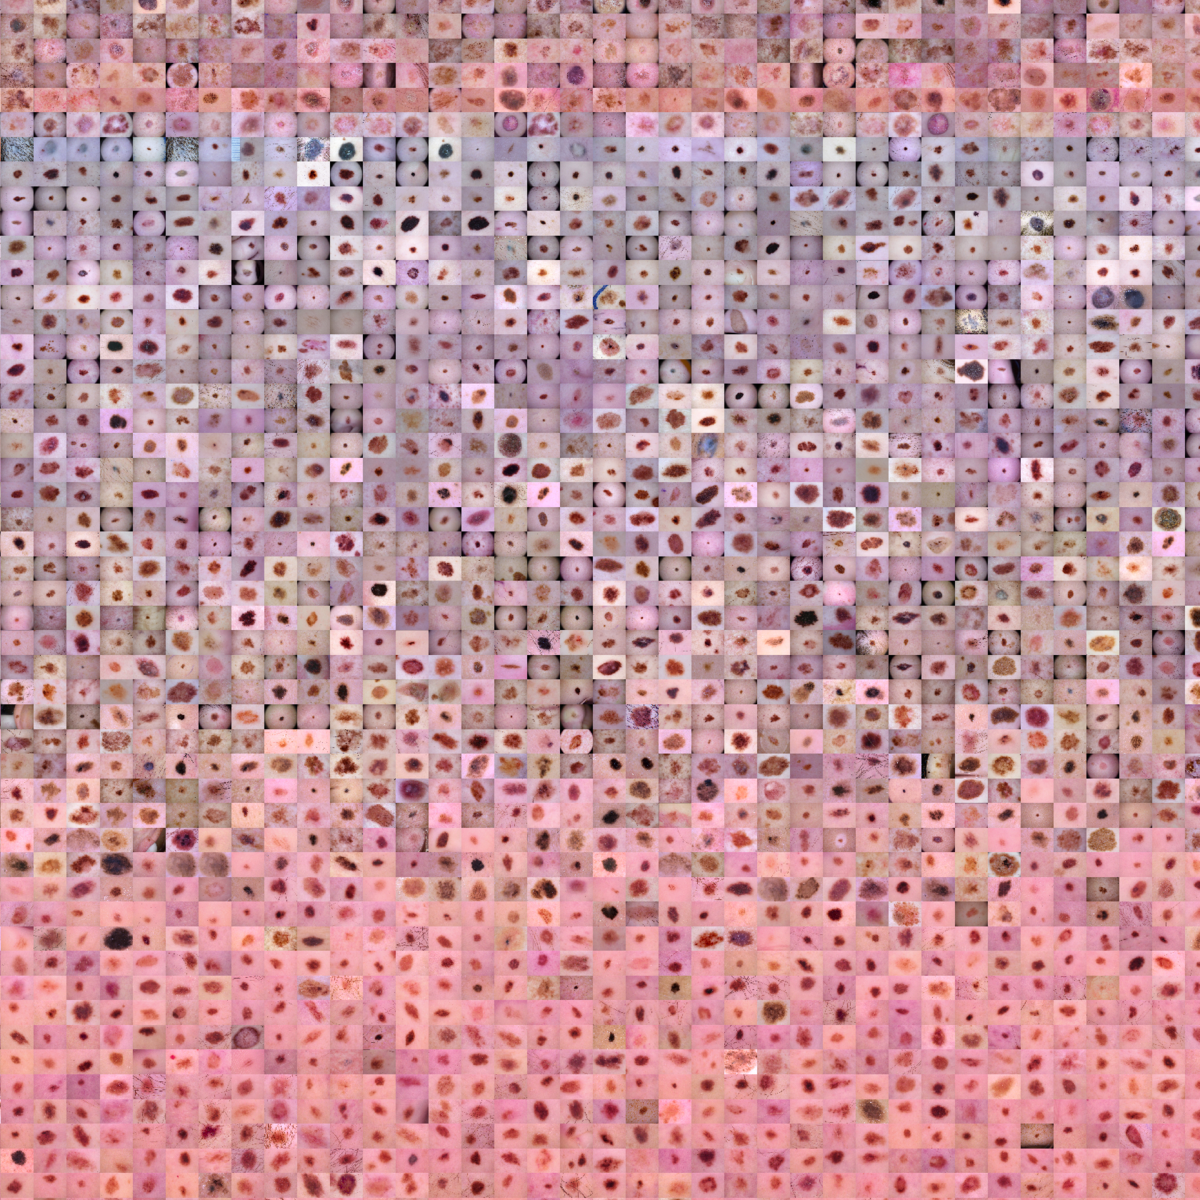
\includegraphics[width=0.25\textwidth]{3/figures/dataset-card.png}
		\caption{Imagén de la Base de Datos. Fuente: \cite{kaggleSkinCancer}}
		\label{1:fig 17}
	\end{center}
\end{figure}





\section{Técnicas para el procesamient y análisis de la información}

\subsection{Metodología de la implementación de la solución}

Para escoger la metodología, se realizó una investigación de las metodologías usadas en los antecedentes presentados con la finalidad de cuál es la que conviene usar más. No obstante, estos solo mencionan los pasas de su metodología, pero no el nombre de este. 

Aun así según la información recolectada se decido implementar la metodología Iterativa. Estas por las siguentes puntos:

- División del trabajo: Permite realizar una división según las partes del proyecto, facilitando la gestión y su seguimiento.

- ttavilidad: Se le puede realizar ajustes si el proyecto lo necesita

\begin{figure}[h]
	\begin{center}
		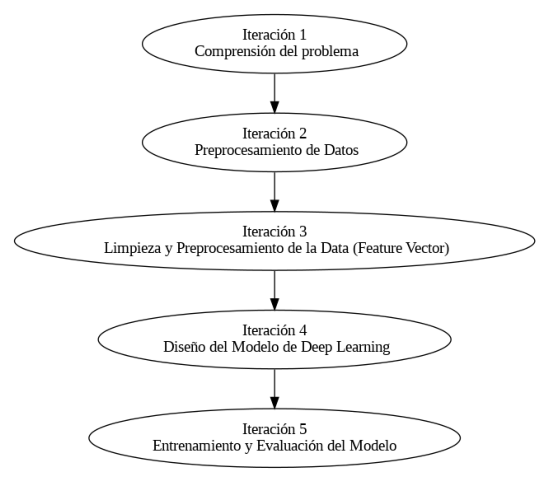
\includegraphics[width=0.5\textwidth]{3/figures/metodologia.png}
		\caption{Imagén de la Base de Datos. Fuente: Elavoracion propia}
		\label{1:fig 19}
	\end{center}
\end{figure}



	






\subsubsection{Metodología para la medición de resultados}

Para evaluar la performance de un modelo, se utilizan diversas métricas como instrumentos de medición de desempeño a partir de los resultados arrojados en la Matriz de confusión. A continuación, se detalla su concepto y sus elementos.


La fórmula de Precisión (Accuracy) se define como:
 
\begin{equation}
	\text{Precisión} = \frac{TP + TN}{TP + TN + FP + FN}
\end{equation}

Esta formula sera usada para la precisio del algoritmo.





\section{Cronograma de actividades}

Se elaboró un cronograma de actividades de toda la investigación, mostrada en la Figura \ref{3:fig13}, contemplando desde el inicio del año 2024 hasta finales del 2024 deonde se realizara la sustentacion del trabajo sustentación del trabajo.

\begin{figure}[h]
	\begin{center}
		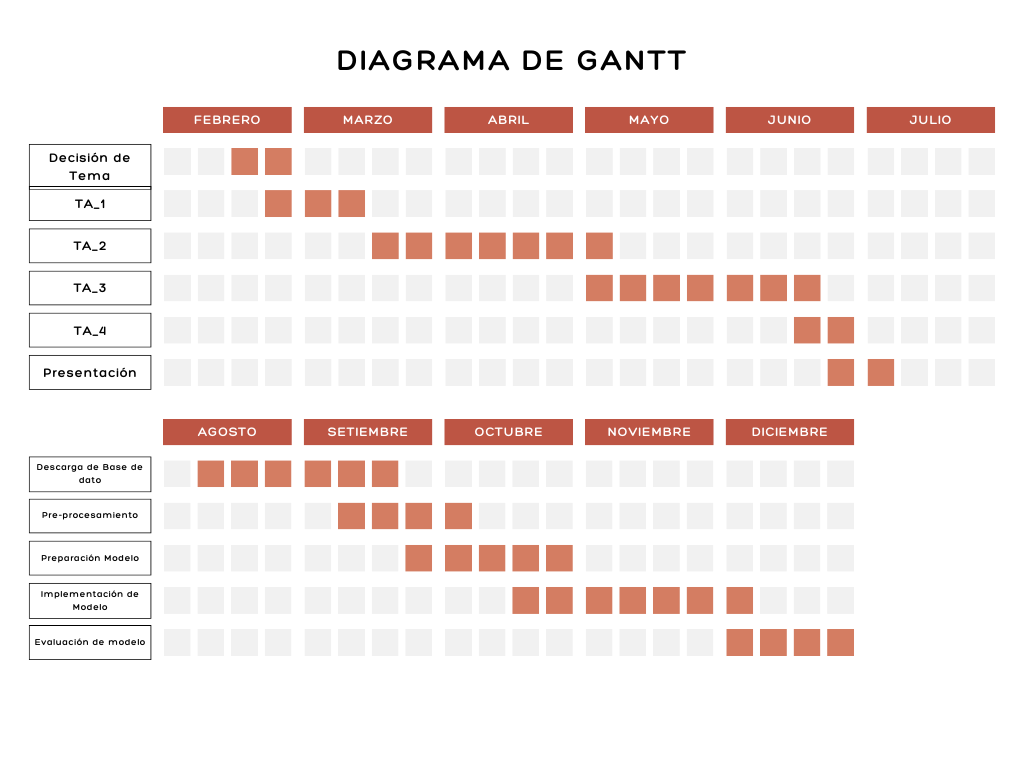
\includegraphics[width=1\textwidth]{3/figures/Cronograma Diagrama de Gantt.png}
		\caption{Diagrama de Grantt. Fuente: Elavoración Propia }
		\label{1:fig 18}
	\end{center}
\end{figure}




\section{Presupuesto}

\begin{center}
	\begin{tabular}{|p{8cm}|p{3cm}|}
		\hline
		Materiales & Costos  \\
		\hline
		Computadora Core i7 & 2000 \\
		\hline

		Total & 2000 \\
		\hline
	\end{tabular}
\end{center}


\begin{comment}
\begin{table}[h!]
	\centering
	\begin{tabular}{|l|p{10cm}|}
		\hline
		\textbf{Concepto} & \textbf{Descripción} \\ \hline
		Población & Personas con lesiones cutáneas, específicamente aquellas que presentan diferentes tipos de cáncer de piel y otras afecciones dermatológicas. \\ \hline
		Muestra & El conjunto de datos contiene un total de 10,015 imágenes de dermatoscopia de lesiones cutáneas. \\ \hline
		Unidad de análisis & Cada imagen de dermatoscopia es una unidad de análisis. Estas imágenes representan diferentes tipos de lesiones cutáneas. \\ \hline
		Variable y tipo de análisis & Clase de la lesión cutánea (melanoma/no melanoma). Clasificación y categorización de las imágenes de acuerdo a los diferentes tipos de lesiones cutáneas. \\ \hline
	\end{tabular}
	
	\label{tabla:dataset}
\end{table}
\end{comment}


\begin{comment}

 Nisi porta lorem mollis aliquam ut porttitor leo. Aenean pharetra magna ac placerat vestibulum. Est placerat in egestas erat imperdiet sed euismod. Velit euismod in pellentesque massa placerat. Enim praesent elementum facilisis leo vel fringilla. Ante in nibh mauris cursus mattis molestie a iaculis. Erat pellentesque adipiscing commodo elit at imperdiet dui accumsan sit. Porttitor lacus luctus accumsan tortor posuere ac ut. Tortor at auctor urna nunc id. A iaculis at erat pellentesque adipiscing commodo elit. La Figura \ref{fig1} y el Cuadro \ref{tab:widgets}

	\begin{figure}[h]
		\begin{center}
			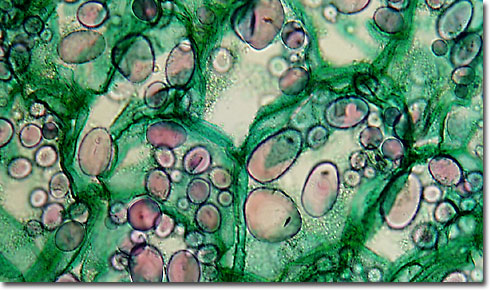
\includegraphics[width=0.8\textwidth]{3/figures/largepotato.jpg}
			\caption{Prueba de Figura}
			\label{fig1}
		\end{center}
		
	\end{figure}


\section{Operacionalización de Variables}

Nisi porta lorem mollis aliquam ut porttitor leo. Aenean pharetra magna ac placerat vestibulum. Est placerat in egestas erat imperdiet sed euismod. Velit euismod in pellentesque massa placerat. Enim praesent elementum facilisis leo vel fringilla. Ante in nibh mauris cursus mattis molestie a iaculis. Erat pellentesque adipiscing commodo elit at imperdiet dui accumsan sit. Porttitor lacus luctus accumsan tortor posuere ac ut. Tortor at auctor urna nunc id. A iaculis at erat pellentesque adipiscing commodo elit.
\section{Instrumentos de medida}
Nisi porta lorem mollis aliquam ut porttitor leo. Aenean pharetra magna ac placerat \begin{itemize}
	\item muscle and fat cells remove glucose from the blood,
	\item cells breakdown glucose via glycolysis and the citrate cycle, storing its energy in the form of ATP,
	\item liver and muscle store glucose as glycogen as a short-term energy reserve,
	\item adipose tissue stores glucose as fat for long-term energy reserve, and
	\item cells use glucose for protein synthesis.
\end{itemize}

\section{Técnicas de recolección de datos}
Nisi porta lorem mollis aliquam ut porttitor leo. Aenean pharetra magna ac placerat vestibulum. Est placerat in egestas erat imperdiet sed euismod. Velit euismod in pellentesque massa placerat. Enim praesent elementum facilisis leo vel fringilla. Ante in nibh mauris cursus mattis molestie a iaculis. Erat pellentesque adipiscing commodo elit at imperdiet dui accumsan sit. Porttitor lacus luctus accumsan tortor posuere ac ut. Tortor at auctor urna nunc id. A iaculis at erat pellentesque adipiscing commodo elit.

\LaTeX{} is great at typesetting mathematics. Let $X_1, X_2, \ldots, X_n$ be a sequence of independent and identically distributed random variables with
\begin{equation}
	S_n = \frac{X_1 + X_2 + \cdots + X_n}{n}
	= \frac{1}{n}\sum_{i}^{n} X_i
	\label{eq1}
\end{equation}

La Ecuación \ref{eq1} denote their mean. Then as $n$ approaches infinity, the random variables $$\sqrt{n}(S_n - \mu)$$ converge in distribution to a normal $\mathcal{N}(0, \sigma^2)$.

\section{Técnicas para el procesamiento y análisis de la información}
Nisi porta lorem mollis aliquam ut porttitor leo. Aenean pharetra magna ac placerat vestibulum. Est placerat in egestas erat imperdiet sed euismod. Velit euismod in pellentesque massa placerat. Enim praesent elementum facilisis leo vel fringilla. Ante in nibh mauris cursus mattis molestie a iaculis. Erat pellentesque adipiscing commodo elit at imperdiet dui accumsan sit. Porttitor lacus luctus accumsan tortor posuere ac ut. Tortor at auctor urna nunc id. A iaculis at erat pellentesque adipiscing commodo elit.

You can make lists with automatic numbering \dots

\begin{enumerate}
	\item Like this,
	\item and like this.
\end{enumerate}
\dots or bullet points \dots
\begin{itemize}
	\item Like this,
	\item and like this.
\end{itemize}


\section{Cronograma de actividades y presupuesto}
Nisi porta lorem mollis aliquam ut porttitor leo. Aenean pharetra magna ac placerat vestibulum. Est placerat in egestas erat imperdiet sed euismod. Velit euismod in pellentesque massa placerat. Enim praesent elementum facilisis leo vel fringilla. Ante in nibh mauris cursus mattis molestie a iaculis. Erat pellentesque adipiscing commodo elit at imperdiet dui accumsan sit. Porttitor lacus luctus accumsan tortor posuere ac ut. Tortor at auctor urna nunc id. A iaculis at erat pellentesque adipiscing commodo elit.

\begin{table}[h]
	\centering
	\begin{tabular}{l|r}
		Item & Quantity \\\hline
		Widgets & 42 \\
		Gadgets & 13
	\end{tabular}
	\caption{\label{tab:widgets}An example table.}
\end{table}

\end{comment}


%\chapter{DESARROLLO DEL EXPERIMENTO}
\section{X}

Hello, here is some text without a meaning.  This text should 
show what a printed text will look like at this place.  If you 
read this text, you will get no information.  Really?  Is there 
no information?  Is there a difference between this text and some 
nonsense like ``Huardest gefburn?  Kjift " not at all!...

\begin{table}
	\centering
	\begin{tabular}{l|r}
		Item & Quantity \\\hline
		Widgets & 42 \\
		Gadgets & 13
	\end{tabular}
	\caption{\label{tab:widgets1}An example table.}
\end{table}

\section{Y}

 Nisi porta lorem mollis aliquam ut porttitor leo. Aenean pharetra magna ac placerat vestibulum. Est placerat in egestas erat imperdiet sed euismod. Velit euismod in pellentesque massa placerat. Enim praesent elementum facilisis leo vel fringilla. Ante in nibh mauris cursus mattis molestie a iaculis. Erat pellentesque adipiscing commodo elit at imperdiet dui accumsan sit. Porttitor lacus luctus accumsan tortor posuere ac ut. Tortor at auctor urna nunc id. A iaculis at erat pellentesque adipiscing commodo elit. 


\section{Z}

Nisi porta lorem mollis aliquam ut porttitor leo. Aenean pharetra magna ac placerat vestibulum. Est placerat in egestas erat imperdiet sed euismod. Velit euismod in pellentesque massa placerat. Enim praesent elementum facilisis leo vel fringilla. Ante in nibh mauris cursus mattis molestie a iaculis. Erat pellentesque adipiscing commodo elit at imperdiet dui accumsan sit. Porttitor lacus luctus accumsan tortor posuere ac ut. Tortor at auctor urna nunc id. A iaculis at erat pellentesque adipiscing commodo elit. 

El paper es citado  y el otro paper .

%\chapter{ANÁLISIS Y DISCUSIÓN DE RESULTADOS}
\section{X}

Hello, here is some text without a meaning.  This text should 
show what a printed text will look like at this place.  If you 
read this text, you will get no information.  Really?  Is there 
no information?  Is there a difference between this text and some 
nonsense like ``Huardest gefburn?  Kjift " not at all!...

\begin{table}
	\centering
	\begin{tabular}{l|r}
		Item & Quantity \\\hline
		Widgets & 42 \\
		Gadgets & 13
	\end{tabular}
	\caption{\label{tab:widgetxcxs}An example table.}
\end{table}

\section{Y}

Nisi porta lorem mollis aliquam ut porttitor leo. Aenean pharetra magna ac placerat vestibulum. Est placerat in egestas erat imperdiet sed euismod. Velit euismod in pellentesque massa placerat. Enim praesent elementum facilisis leo vel fringilla. Ante in nibh mauris cursus mattis molestie a iaculis. Erat pellentesque adipiscing commodo elit at imperdiet dui accumsan sit. Porttitor lacus luctus accumsan tortor posuere ac ut. Tortor at auctor urna nunc id. A iaculis at erat pellentesque adipiscing commodo elit. 


\section{Z}

Nisi porta lorem mollis aliquam ut porttitor leo. Aenean pharetra magna ac placerat vestibulum. Est placerat in egestas erat imperdiet sed euismod. Velit euismod in pellentesque massa placerat. Enim praesent elementum facilisis leo vel fringilla. Ante in nibh mauris cursus mattis molestie a iaculis. Erat pellentesque adipiscing commodo elit at imperdiet dui accumsan sit. Porttitor lacus luctus accumsan tortor posuere ac ut. Tortor at auctor urna nunc id. A iaculis at erat pellentesque adipiscing commodo elit.

%\chapter{CONCLUSIONES Y RECOMENDACIONES}
\section{Conclusiones}

Hello, here is some text without a meaning.  This text should 
show what a printed text will look like at this place.  If you 
read this text, you will get no information.  Really?  Is there 
no information?  Is there a difference between this text and some 
nonsense like ``Huardest gefburn?  Kjift " not at all!...



\section{Recomendaciones}

Nisi porta lorem mollis aliquam ut porttitor leo. Aenean pharetra magna ac placerat vestibulum. Est placerat in egestas erat imperdiet sed euismod. Velit euismod in pellentesque massa placerat. Enim praesent elementum facilisis leo vel fringilla. Ante in nibh mauris cursus mattis molestie a iaculis. Erat pellentesque adipiscing commodo elit at imperdiet dui accumsan sit. Porttitor lacus luctus accumsan tortor posuere ac ut. Tortor at auctor urna nunc id. A iaculis at erat pellentesque adipiscing commodo elit. 



%%Anexos
\appendix
\renewcommand{\appendixname}{Anexos}
\renewcommand{\appendixtocname}{Anexos}
\renewcommand{\appendixpagename}{Anexos}
\clearpage
\addappheadtotoc
\appendixpage
\chapter{Anexo I: Árbol de Problema }

\begin{figure}[h]
	\begin{center}
		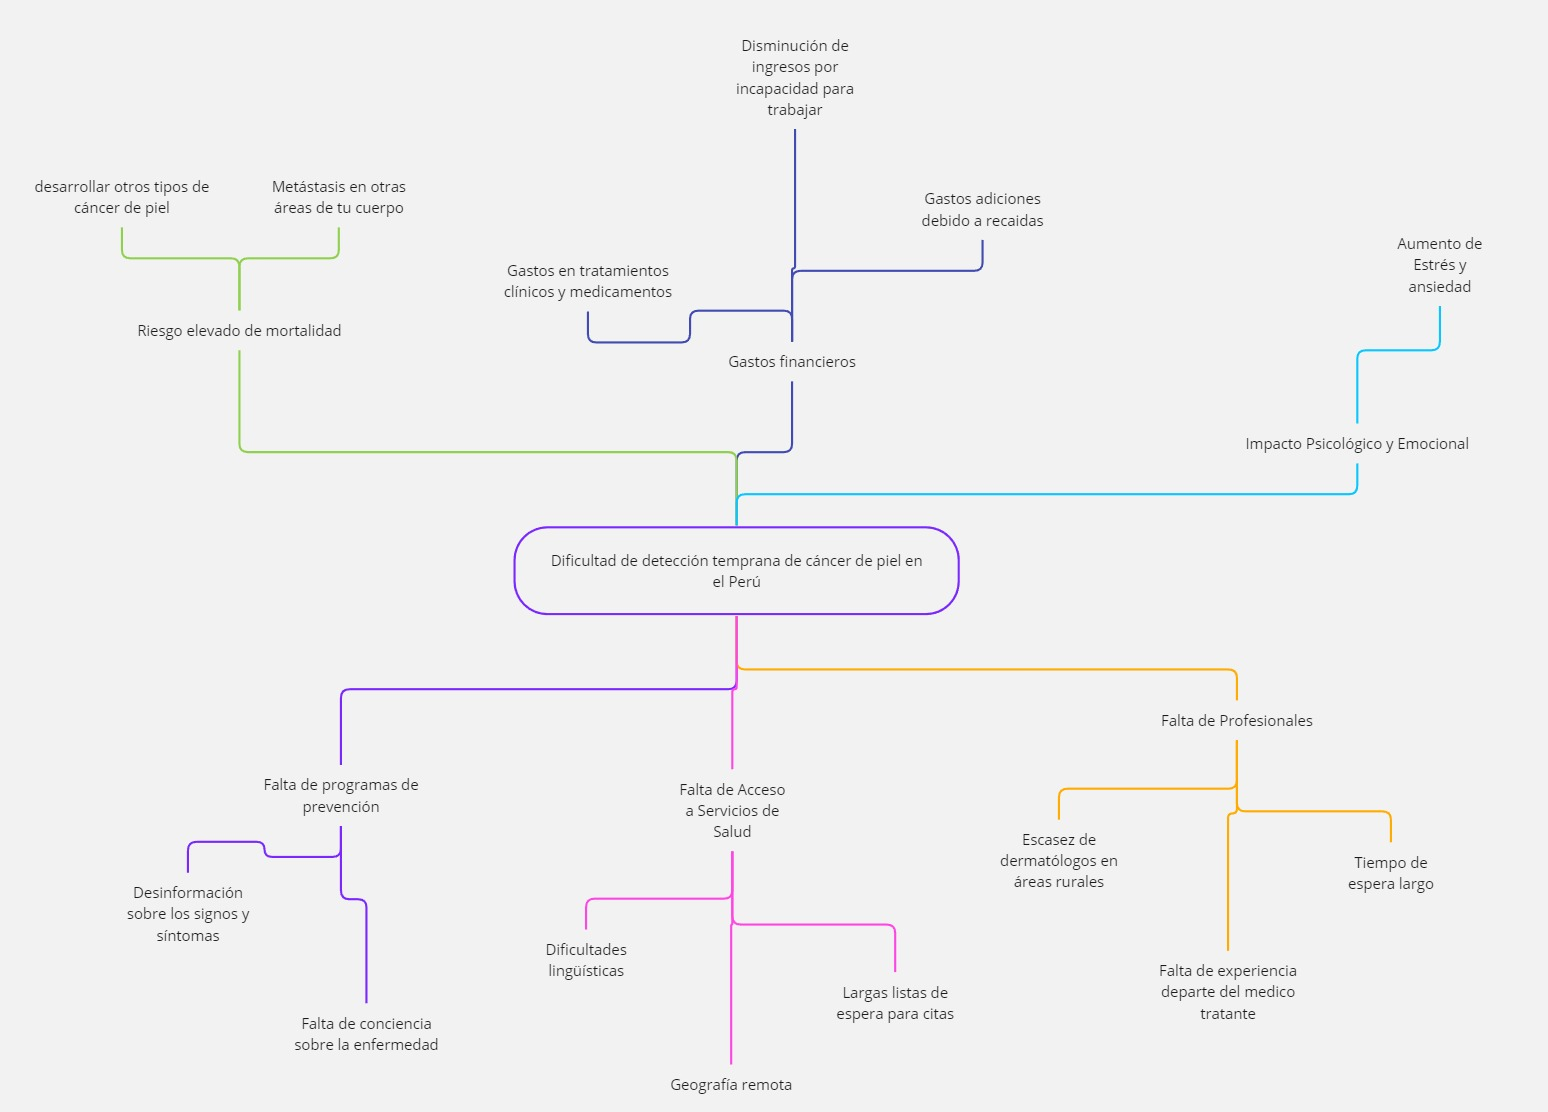
\includegraphics[width=0.8\textwidth]{images_repo/Anexo/Problem Tree Template.jpg}
		\caption{Árbol de Problema. Fuente: Elaboración propia}
		\label{1:arbolProblema}
	\end{center}
\end{figure}



\chapter{Anexo II: Árbol de Objetivo}

\begin{figure}[h]
	\begin{center}
		\includegraphics[width=0.8\textwidth]{images_repo/Anexo/Árbol de Objetivos.jpg}
		\caption{Árbol de Problema. Fuente: Elaboración propia}
		\label{1:arbolObjeti}
	\end{center}
\end{figure}



\chapter{Anexo II: Matriz de Consistencia}


\begin{table}[h!]
	\centering
	\small
	\begin{tabular}{ |m{5cm}|m{5cm}|m{5cm}|  }
		\hline
		\rowcolor{bluejean}
		\Centering \color{white}{PROBLEMAS}& \Centering \color{white}{OBJETIVOS}& \Centering \color{white}{HIPÓTESIS}\\
		\hline
		\rowcolor{turq}
		\Centering Problema General& \Centering Objetivo General & \Centering Hipótesis General \\
		\hline
		{\ProblemaGeneral} & { \ObjetivoGeneral} & {\HipotesisGeneral} \\
		\hline
		\rowcolor{turq}
		\Centering Problemas Específicos& \Centering Objetivos Específicos & \Centering Hipótesis Específicas \\
		\hline
		{\Pbone} & {\Objone} & {\Hone} \\
		\hline
		{\Pbtwo} & {\Objtwo} & {\Htwo} \\
		\hline
		{\Pbthree} & {\Objthree} & {\Hthree} \\
		\hline
		{\Pbfour} & {\Objfour} & {\Hfour} \\
		\hline
	\end{tabular}
	\caption{Matriz de consistencia. Fuente: Elaboración propia}
	\label{1:table}
\end{table}


\begin{figure}[h]
	\begin{center}
		\includegraphics[angle=90, width=0.8\textwidth]{images_repo/Anexo/Matriz.png}
		\caption{Matriz de consistencia con Indicadores. Fuente: Elaboración propia}
		\label{1:Matriz de consistencia }
	\end{center}
\end{figure}



\chapter{Anexo II: Resumen de Papers investigados}
%\section{Conclusiones}

\begin{table}[h]
	\newcommand{\multirot}[1]{\multirow{2}{*}[-8ex]{\rotcell{\rlap{#1}}}}
	%\scriptsize
	\footnotesize
	\centering
	\begin{longtable}{|m{0.5cm}|m{0.3cm}|m{4cm}|m{2cm}|m{0.6cm}|m{1.7cm}|m{3cm}|} 
		\hline
		\rowcolor[rgb]{0,0.251,0.502} \multicolumn{1}{|c|}{\textcolor{white}{Tipo}} & \multicolumn{1}{c|}{\textcolor{white}{N°}} & \multicolumn{1}{c|}{\textcolor{white}{Título}}                                                                             & \multicolumn{1}{c|}{\textcolor{white}{Autor}}        & \multicolumn{1}{c|}{\textcolor{white}{Año}} & \multicolumn{1}{c|}{\textcolor{white}{País}} & \multicolumn{1}{c|}{\textcolor{white}{Fuente}}                                                        \\ 
		\hline
		\multirot{Problema}                                        & 1                                             & Deep Learning-Based Transfer Learning for Classification of Skin Cancer~                                                                               & Satin, J. , Udit, S., Balakrushna, T., Emad, A. Mohamed K. and Ali K. & 2021 &  Arabia Saudita. & Sensors \\ 
		\cline{2-7}
		& 2& Skin cancer classification via convolutional neural networks systematic review of studies involving human experts & S. Haggenmu ller, A. Hekler, R.C. Maron, V.M. Rotemberg& 2021& Europa& European Journal of Cancer \\ 
		\hline
		\multirow{3}{*}[-14ex]{\rotcell{\rlap{Propuesta}}}
		& 3                                             & An enhanced technique of skin cancer classification using deep convolutional neural network with transfer learning models~                                                                               & Md Shahin Ali, Md Sipon Miah, Jahurul Haque, Md Mahbubur Rahman y Md Khairul Islam                                 & 2021                                        &  República de Irlanda         & Machine Learning with Applications, 2021, vol. 5                                                                  \\ 
		\cline{2-7}
		& 4 & Design of a tool for the classification of skin cancer imagesVTusing Deep Neural Networks (DNN) & Diana Paola Merchan Vargas, Helis Navarro Baez, Jaime Guillermo Barrero Perez y Jeyson Arley Castillo Bohórquez   & 2021& Argentina       & Ciencia y Tecnologia, numero 21 del año 2021.                                                    \\ 
	
		
		\hline
	\end{longtable}
	\caption{Cuadro Resumen de Papers investigados. Parte I. Fuente: Elaboración propia}
\label{A:table}
\end{table}


\begin{table}[h]
	\newcommand{\multirot}[1]{\multirow{2}{*}[-8ex]{\rotcell{\rlap{#1}}}}
	%\scriptsize
	\footnotesize
	\centering
	\begin{longtable}{|m{0.5cm}|m{0.3cm}|m{4cm}|m{2cm}|m{0.6cm}|m{1.7cm}|m{3cm}|} 
		\hline
		\rowcolor[rgb]{0,0.251,0.502} \multicolumn{1}{|c|}{\textcolor{white}{Tipo}} & \multicolumn{1}{c|}{\textcolor{white}{N°}} & \multicolumn{1}{c|}{\textcolor{white}{Título}}                                                                             & \multicolumn{1}{c|}{\textcolor{white}{Autor}}        & \multicolumn{1}{c|}{\textcolor{white}{Año}} & \multicolumn{1}{c|}{\textcolor{white}{País}} & \multicolumn{1}{c|}{\textcolor{white}{Fuente}}                                                        \\ 
		
		\hline
		\multirow{4}{*}[-28ex]{\rotcell{\rlap{Técnica}}}                                          
		& 5                                             & Diagnosis of skin cancer using machine learning techniques                                               &A. Murugan, S. Anu H. Nair y K.P. Sanal Kumar & 2021                                        & India                                          & Microprocessors and Microsystems en 2021             \\ 
		\cline{2-7}
		
		
		
		
		& 6                                             & Multiclass skin cancer classification using EfficientNets – a first step towards preventing skin cancer~                   & K. Ali, Z.A. Shaikh, A.A. Khan, S. Rathod, S. Das                                      & 2022                                        & Pakistan                                        & 2022, revista Neuroscience Informatics \\ 
		\cline{2-7}
		& 7                                             & Skin cancer classification using explainable artificial intelligence on pre-extracted image features & Khater, T., Ansari, S., Mahmoud, S., Hussain, A., Tawfik, H. & 2017 & Miratos Árabes Unidos          & revista "Intelligent Systems with Applications" en el año 2023
		Association of Automation (YAC)~              \\ 
		\cline{2-7}
		& 8                                             & An improved transformer network for skin cancer classification
		&  C. Xin, Y. Wang, G. Wang, X. Zhao, Y. Dong y M. Lu.~             & 2022                                        & China                                          & Computers in Biology and Medicine              \\ 
		\cline{2-7}
		& 9                                             & Uncertainty quantification in skin cancer classification using three-way decision-based Bayesian deep learning                                                                      & M. Abdar, F. Pourpanah, S. Hussain, D. Rezazadegan, L. Liu, M. Ghavamzadeh, P. Fieguth, X. Cao, A. Khosravi y U.R. Acharya                                   & 2021                                        & -                                          & Computers in Biology and Medicine                          \\
		\cline{2-7}
		& 10                                             &A multi-class skin Cancer classification using deep convolutional neural networks    & Saket S. Chaturvedi, Jitendra V. Tembhurne, Tausif Diwan2 & 2020                               & -         & Springer Science+Business Media, LLC, part of Springer Nature 2020 \\
		\hline
	\end{longtable}
	\caption{Cuadro Resumen de Papers investigados. Parte II. Fuente: Elaboración propia}
	\label{A:table}
\end{table}




% %%Bibliografia
%\bibliographystyle{apalike} % Title is link if provided
%\renewcommand{\bibname}{BIBLIOGRAFÍA} % changes the header; default: Bibliography

\printbibliography[heading=bibintoc,title={BIBLIOGRAFÍA}]
%\bibliography{biblio/references} % adjust this to fit your BibTex file
\end{document}